\documentclass[12pt,a4paper]{report}

\setcounter{secnumdepth}{3} %The level of sections that get numbered
\setcounter{tocdepth}{3} %The level of sections to appear in ToC
\usepackage{url}
\usepackage{lscape}
\usepackage{graphicx}
\usepackage{pdfpages}
\usepackage{listings}
\usepackage{setspace}
\usepackage[numbers]{natbib}
\usepackage{amsfonts} % This package is needed for \mathbb
\usepackage{float}
\usepackage[hidelinks]{hyperref}
\usepackage{amsmath}
\usepackage{subcaption}
\usepackage{multirow}
\usepackage{colortbl}
\usepackage{xcolor}
\usepackage{diagbox}



%Date formatting Package
\usepackage[ddmmyyyy]{datetime}

\usepackage{wrapfig}


\begin{document}
\begin{titlepage} \vspace{1cm}

\begin{center}
\textbf{\Huge Generating images using a Deep Convolutional GANs}
\end{center}

\vspace{1.0cm}

\begin{figure}[h]
    \centering
    
\includegraphics[scale = 0.7]{Images/UCC_logo} 
\end{figure}

\vspace{1.0cm}

\begin{center}
\textbf{\Large Author:} \Large{Kai Deng} {\LARGE\par}
\textbf{\Large Supervisor:} \Large{Serhiy Yanchuk} {\LARGE\par}
\end{center}
\vspace{1.0cm}

\begin{center}
\Large
A thesis submitted in partial fulfilment of the requirements for the degree of\\ MSc Mathematical Modelling and Machine Learning
\vfill{}
\Large{School of Mathematical Sciences, \\
University College Cork, \\
Ireland \\
\vspace{0.4cm}
September 2024}
\end{center}

\end{titlepage}

\onehalfspacing

\chapter*{Declaration of Authorship}

This report is wholly the work of the author, except where explicitly
stated otherwise. The source of any material which was not created
by the author has been clearly cited. \\
\medskip{}

\textbf{Date:} \quad \today

\medskip{}

\textbf{Signature: Kai Deng} 

\chapter*{Acknowledgements}

I would like to express my deepest gratitude to my supervisor, Professor Serhiy Yanchuk, 
for his invaluable guidance, continuous support, and insightful feedback throughout the 
course of my research. His expertise and encouragement have been instrumental in the 
successful completion of this thesis.

\begin{abstract}
    Generative Adversarial Networks (GANs) have become a pivotal tool in the field of generative modeling, 
    offering a novel approach to generating realistic data through the adversarial training of a generator 
    and a discriminator. This thesis investigates the performance of GANs in generating high-quality images, 
    with a particular focus on the challenges associated with model structure, training stability, and evaluation metrics.
    
    In this study, I employed the Animal Faces-HQ (AFHQ) dataset, consisting of 16,130 high-resolution images, 
    to train a standard GAN model aimed at generating realistic cat images. The research explored the impact of
     various architectural choices, including the use of convolutional layers versus dense layers, as well as 
     the effects of data augmentation techniques on model performance. The experiments revealed that convolutional 
     architectures significantly outperformed dense ones, highlighting the importance of spatial feature extraction
     in image generation tasks.
    
    The study also examined the role of data augmentation in GAN training, finding that while augmentation can 
    introduce useful variability into the training data, it may also lead to optimization challenges if not carefully 
    applied. The final model, trained on downscaled images due to hardware limitations, was able to produce highly 
    realistic cat images, demonstrating the effectiveness of GANs in high-resolution image synthesis.
    
    The findings contribute to a deeper understanding of how GAN architecture and training strategies influence 
    the quality of generated images, offering insights for future research and practical applications in fields 
    requiring high-quality image generation. The study concludes by suggesting directions for further exploration, 
    including the potential benefits of more advanced GAN variants and higher-resolution training data.
\end{abstract}

\tableofcontents{}

\listoffigures{}

\newpage
\chapter{Introduction}


Generative Adversarial Networks (GANs) have emerged as a transformative tool in generative modeling, framing the problem as a competition between two networks: a generator that creates synthetic data from noise, and a discriminator that differentiates between real and generated data \citep{10.48550/arxiv.1704.00028}. Since their introduction in 2014, GANs have found applications in fields such as materials science, radiology, and computer vision \citep{10.1002/mgea.30}, \citep{10.1016/j.media.2019.101552}, \citep{10.1016/j.artmed.2020.101938}. For instance, CycleGAN has been applied in medical imaging, enhancing tasks like liver lesion classification through synthetic image augmentation, outperforming traditional methods in sensitivity and specificity \citep{10.1016/j.neucom.2018.09.013}. Similarly, StyleGAN has shown effectiveness in image deformation and style transfer \citep{10.1109/iccv.2019.00453}, further expanding the reach of GANs in the computer vision field, where they generate data without explicitly modeling probability density functions \citep{10.1016/j.media.2019.101552}.

However, despite their success, training GANs presents notable challenges, including issues like mode collapse, training instability, and the high computational demands required for effective performance. Evaluating GANs is also complex, as traditional metrics such as accuracy are insufficient to measure the quality and diversity of generated data. These difficulties have driven the development of various architectures and training methods aimed at improving the stability and effectiveness of GANs.

The objective of this thesis is to contribute to a clearer understanding of the factors that influence GAN performance, particularly in generating realistic images. For this purpose, I use the Animal Faces-HQ (AFHQ) dataset, containing 16,130 high-resolution images at 512×512 pixels, to train a GAN model specifically for generating realistic cat images. The high resolution presents both opportunities and challenges, as it requires careful attention to the model’s architecture and training to avoid overfitting or underfitting.

This thesis is organized as follows: Chapter 2 provides an overview of previous models for image generation, including Deep Boltzmann Machines, Variational Autoencoders, and Noise Contrastive Estimation. Chapter 3 covers the theoretical background of GANs, focusing on their objective functions, training dynamics, and performance evaluation. Chapter 4 describes the experimental work, including model selection, architectural exploration, and the impact of data augmentation, along with the application of the GAN model to the AFHQ dataset and then presents the results, discusses their implications, and suggests potential avenues for future research.


\newpage
\chapter{Historical Models of Image Generation}
\label{Related Work}


This chapter reviews key historical models of image generation, including Deep Boltzmann Machines (DBMs), 
Variational Autoencoders (VAEs), and Noise Contrastive Estimation (NCE). Each of these models has contributed 
to the development of generative modeling by introducing different approaches to learning data distributions. 

\section{Deep Boltzmann Machines}

Deep Boltzmann Machines (DBMs) are sophisticated generative models that excel in learning intricate data representations 
in an unsupervised manner. Unlike traditional feedforward networks, DBMs are structured with multiple layers of stochastic, 
binary latent variables, where each layer captures progressively abstract features of the input data. This architecture is 
characterized by fully connected layers, with no direct connections between units within the same layer, which enables DBMs 
to effectively model complex dependencies inherent in the data \citep{10.1007/978-3-642-40728-4_14}. The undirected nature 
of the connections in DBMs allows for the propagation of uncertainties across layers, enhancing their capability in feature 
learning and unsupervised pre-training \citep{10.1007/978-3-642-40728-4_14}\citep{10.48550/arxiv.1203.3783}.

However, the training of DBMs presents significant challenges, primarily due to their reliance on Markov Chain Monte Carlo (MCMC) methods, 
such as Gibbs sampling, for approximate inference. These methods are essential for estimating gradients and the intractable partition 
function, which is vital for updating model parameters. The computational overhead introduced by MCMC methods often results in 
slow convergence and increased complexity, particularly when applied to large-scale datasets \citep{10.48550/arxiv.2303.10728}. 
The requirement for numerous sampling steps to achieve equilibrium further complicates the training process, making DBMs less 
accessible compared to other generative models, such as Variational Autoencoders (VAEs).

To mitigate these training difficulties, DBMs often utilize layer-wise pre-training, which initializes model parameters 
before the entire network is fine-tuned. This approach has been shown to enhance the efficiency of the learning process
by providing a sensible initialization for the weights and variational inference \citep{10.1162/neco_a_00311}. Despite 
these strategies, the inherent complexity associated with MCMC methods continues to pose challenges in scaling DBMs 
effectively, particularly in comparison to more straightforward generative models like VAEs \citep{10.48550/arxiv.2303.10728}. 
Recent advancements have explored alternative training methodologies, including the use of specialized hardware systems to improve 
the efficiency of sampling tasks, thereby addressing some of the computational hurdles associated with traditional training approaches \citep{10.48550/arxiv.2303.10728}.



\section{Variational Autoencoders}
Variational Autoencoders (VAEs) are generative models in machine learning that excel in tasks like image generation and data 
representation by learning the underlying structure of data through a latent space. 

The architecture of VAEs consists of an encoder that maps input data into a latent space, where the latent variables are 
typically assumed to follow a Gaussian distribution. This assumption simplifies the learning process, as it allows for 
the use of techniques such as the reparameterization trick, which enables backpropagation through stochastic layers \citep{10.1561/2200000056}. 
The decoder then reconstructs the input data from the latent variables, ensuring that the model captures the essential 
features of the data distribution. The loss function of a VAE combines reconstruction loss with a Kullback-Leibler (KL) 
divergence term, which regularizes the latent space and encourages the model to learn a smooth and continuous representation \citep{10.3390/jimaging4020036}.

In comparison to DBMs, VAEs offer several advantages, including simpler training dynamics and better scalability. DBMs 
often require complex sampling methods, such as Gibbs sampling, which can be computationally intensive and slow to converge. 
In contrast, VAEs can be trained using standard gradient descent methods, making them more accessible for 
practitioners \citep{10.1561/2200000056}\citep{10.1109/access.2020.2977671}. Furthermore, the structured latent space of 
VAEs not only allows for efficient sampling but also supports various applications, such as image generation, anomaly detection, 
and data imputation, where the ability to interpolate between data points is crucial \citep{10.1088/2632-2153/ab80b7}\citep{10.48550/arxiv.2002.10464}.

However, VAEs face limitations in modeling discrete data as they require back-propagation through hidden units, which poses challenges 
in handling such data types effectively \citep{10.48550/arxiv.1909.13062}. Despite this limitation, VAEs have been extensively used to 
represent high-dimensional complex data by learning a low-dimensional latent space in an unsupervised manner \citep{10.48550/arxiv.2106.06500}.


\section{Noise Contrastive Estimation}


Noise-Contrastive Estimation (NCE) is a statistical method employed in machine learning, particularly for estimating parameters of unnormalized probabilistic models. The fundamental principle of NCE is to recast the maximum likelihood estimation problem into a binary classification task. In this framework, the model is trained to differentiate between actual data samples and artificially generated noise samples, which are drawn from a known distribution \citep{10.48550/arxiv.1711.00658}. This transformation simplifies the estimation process and circumvents the computational challenges associated with calculating the intractable partition function, a common hurdle in traditional maximum likelihood estimation methods for unnormalized models \citep{10.48550/arxiv.2110.11271}.

The methodology of NCE involves the introduction of noise samples, which serve as a baseline for comparison against real data. The model is trained to assign higher probabilities to genuine data samples while assigning lower probabilities to noise samples. This approach effectively enables the model to learn the underlying data distribution without the necessity of explicit normalization \citep{10.21437/interspeech.2016-1295}. The binary classification framework utilized in NCE allows for the application of standard logistic regression techniques, enhancing both the tractability and computational efficiency of the training process \citep{10.18653/v1/e17-2003}. Moreover, NCE has been shown to be particularly advantageous in large-scale models, such as energy-based models and word embeddings, where the computational burden of normalization can be substantial \citep{10.48550/arxiv.2101.03288}.

Despite its advantages, NCE is not without limitations. The choice of noise distribution is critical to the performance of the model; poorly selected noise distributions can lead to suboptimal parameter estimates and slow convergence rates \citep{10.48550/arxiv.2110.11271}. Additionally, while NCE simplifies the training of unnormalized models, it may not perform as effectively in scenarios where the noise distribution is challenging to define or when dealing with highly complex data distributions. The empirical observations regarding the importance of noise distribution have been formalized in various studies, underscoring the need for careful consideration in its selection \citep{10.48550/arxiv.2110.11271}.



\newpage
\chapter{Theoretical Background}
\label{Theoretical Background for GAN}

\section*{Generative Adversarial Nets}

Generative Adversarial Networks (GANs) consist of a generator G and a discriminator D, 
both implemented using artificial neural networks. The parametrization of GANs involves 
defining the network structure of these components and initializing their weights and biases \citep{10.1007/s10928-021-09787-4}. 
The success of GANs relies on balancing the training of these two networks, where the 
G aims to produce samples $G(z)$ that mimic real data distributions $p_{data}(x)$ by input noise z, while the D 
learns to differentiate between real and generated samples \citep{10.1109/taslp.2017.2761547}. 
The training process involves iteratively updating the weights and biases of the networks through 
adversarial training, where the generator tries to deceive the discriminator, and the discriminator 
aims to accurately classify samples \citep{10.48550/arxiv.1802.05637}.
The formula 3.1 is the objective function of Generative Adversarial Networks (GANs):

\begin{equation}
    \min_{G} \max_{D} V(D, G) = \mathbb{E}_{x \sim p_{data}(x)} [\log D(x)] + \mathbb{E}_{z \sim p_{z}(z)} [\log(1 - D(G(z)))].
\end{equation}



It describes the game process between the Generator (G) and the Discriminator (D). Specifically, the formula defines a minimax game between the Discriminator and the Generator.

\begin{itemize}
    \item \textbf{ $D(G(z))$:} is the output of the discriminator for the data G(z) generated by the generator. Indicating the probability that the discriminator believes that the generated data comes from the real data distribution.
    \item \textbf{$D(x)$:} is the output of the discriminator for the real data x. Indicating the probability that the discriminator believes that the real data x comes from the real data distribution.
    \item \textbf{ $x \sim p_{data}(x)$:} means that sample x is drawn from the true data distribution $p_{data}$.
    \item \textbf{ $z \sim p_{z}(z)$:} means that sample z is drawn from the fake data distribution $p_{z}$.
    \item \textbf{$\mathbb{E}{_x \sim p_{data}(x)}[\log D(x)]$:} means taking the average value of $\log D(x)$ for all samples x on the true data distribution $p_{data}(x)$.
    \item \textbf{$\mathbb{E}{x \sim p_{z}(z)}[\log (1 - D(x))]$:} means taking the average value of $\log (1 - D(G(z)))$ for all samples z on the noise distribution $p_z(z)$.
\end{itemize}




D(G(z)) is the output of the discriminator for the data G(z) generated by the generator, 
indicating the probability that the discriminator believes that the generated data comes from the real data distribution.
D(x) is the output of the discriminator for the real data x, 
indicating the probability that the discriminator believes that the real data x comes from the real data distribution.

$\mathbb{E}{x \sim p_{data}(x)}[\log D(x)]$ represents the average value of $\log D(x)$ for all samples x on the true data distribution $p_{data}(x)$.
$x \sim p_{data}(x)$ means that sample x is drawn from the true data distribution $p_{data}$.
$\log D(x)$ is the logarithm of the output of the discriminator D for the input x.


\begin{equation}
    \max_{D} V(D, G) = \mathbb{E}_{x \sim p_{data}(x)} [\log D(x)] + \mathbb{E}_{z \sim p_{z}(z)} [\log(1 - D(G(z)))].
\end{equation}

The formula 3.2 shows, the discriminator tries to maximize V(D, G).

\begin{equation}
    \min_{G} V(D, G) = \mathbb{E}_{z \sim p_{z}(z)} [\log(1 - D(G(z)))].
\end{equation}


The formula 3.3 shows, the generator tries to minimize V(D, G). 
This means that the generator tries to generate realistic data G(z) so that the discriminator cannot distinguish 
them from real data, that is: It is hoped that D(G(z)) is close to 1, so that $\log (1 - D(G(z)))$ is closer to negative infinity.
This dynamic equilibrium drives the GAN framework towards generating outputs that closely resemble authentic data, 
fulfilling the objective of producing realistic data that is challenging to distinguish from real data.


\begin{equation}
    \min_{G} V(D, G) = \mathbb{E}_{z \sim p_{z}(z)} [-\log(D(G(z)))].
\end{equation}

In real training process, the formula 3.3 will replace by 3.4. Since, when the discriminator D is strong, 
the gradient of the $log(1 - D(G(z)))$ approaches zero, leading to slow generator training and diminished gradient update impact \citep{10.1007/s11263-019-01265-2}.  
This approach ensures that the gradient of the logarithm is large, providing the generator with more effective gradient updates and 
helping to avoid the vanishing gradient issue \citep{10.1109/tpami.2018.2872043}.



The GAN network parameters play a crucial role in determining the quality and diversity of 
the generated samples $G(x)$ \citep{10.1007/s10928-021-09787-4}. The optimization process in GANs 
typically involves minimizing a min-max function to ensure the G produces samples that 
are indistinguishable from real data \citep{10.1109/taslp.2017.2761547}. Maintaining this balance 
during training is essential for achieving high-quality sample generation \citep{10.1007/s10928-021-09787-4}. 
The D's role is to provide feedback to the generator by acting as a critic, 
guiding the G towards producing more realistic samples \citep{10.48550/arxiv.1802.05637}.



\section*{Optimal Discriminator}

The training process of Generative Adversarial Networks (GANs) is inherently adversarial. 
The generator endeavors to create increasingly realistic fake samples to deceive the discriminator, 
while the discriminator seeks to more accurately distinguish between real and fake samples. 
To understand how this process works, in the following sections, 
I will describe the GAN training process from the perspectives of data distribution and mathematical formulation.

\subsection*{Distribution Angle}



\begin{figure}[H]
    \centering
    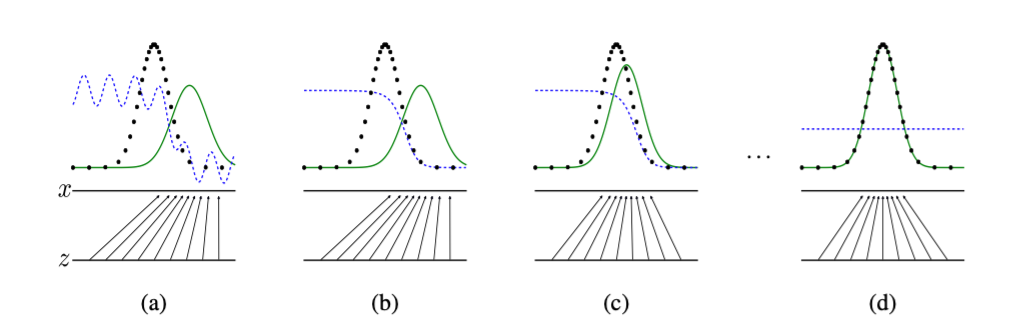
\includegraphics[width=1.2\linewidth]{./Images/data_distribution.jpg}
    \caption{Diagram of GAN training process}
    \label{fig:my_picture}
    \vspace{1pt} % Vertical space, optional
    \small{Source: \cite{goodfellow2014generative}}
\end{figure}


\begin{itemize}
    \item \textbf{ Green Curve:} Represents the distribution of generated samples. Initially, the distribution of generated samples may differ significantly from the real samples. As training progresses, the generated samples’ distribution gradually approaches that of the real samples.
    \item \textbf{Black Dots:} Represent the distribution of real samples. These points remain unchanged throughout the training process and represent the target distribution.
    \item \textbf{ Blue Line:} Represents error or noise. Initially, the error is large and manifests as a wavy sine curve. As training progresses, the error gradually decreases, and the blue line becomes increasingly flat.
    \item \textbf{ Lines Arranged Below (Labeled as x and z):} Represent the distribution of samples in the latent space. In GAN training, samples from the latent space are mapped to the data space through the generator, producing corresponding samples.
\end{itemize}


During the training process of the GAN model, the generator and the discriminator fight against each other. 
The generator tries to produce realistic samples to fool the discriminator, while the discriminator strives 
to distinguish real samples from generated samples. Initially, the generator generates samples with poor 
quality and large errors, similar to the blue sine wave in Figure (a). However, as training proceeds and 
the generator continues to improve, the error in generated samples gradually decreases, similar to the 
blue lines in figures (b) and (c) becoming flat. At the same time, the distribution of real samples and 
generated samples gradually becomes consistent, and finally reaches the optimal state in Figure (d). At this moment $p_{data}(x) = p_g(x)$, 
the samples generated by the generator are almost the same as the real samples, and the error is minimized. 
During the entire process, the sample distribution gradually converges from the initial noise and discrete 
state to a state that highly coincides with the real distribution, reflecting a significant improvement in 
the quality of the generated samples.


\subsection*{Formula Angle}


1. Problem Setup

In a Generative Adversarial Network (GAN), the objective is to train a generator \( G \) and a discriminator \( D \) to generate data that resembles the real data distribution. The objective function to be maximized is given by:

\begin{equation}
    V(D, G) = \mathbb{E}_{\mathbf{x} \sim p_{\text{data}}(\mathbf{x})} [\log D(\mathbf{x})] + \mathbb{E}_{\mathbf{z} \sim p_{\mathbf{z}}(\mathbf{z})} [\log (1 - D(G(\mathbf{z})))].
\end{equation}

2. Rewriting the Objective Function

First, the objective function is rewritten in integral form:

\begin{equation}
    V(D, G) = \int p_{\text{data}}(\mathbf{x}) \log D(\mathbf{x}) \, d\mathbf{x} + \int p_{\mathbf{z}}(\mathbf{z}) \log (1 - D(G(\mathbf{z}))) \, d\mathbf{z}.
\end{equation}

By changing variables \(\mathbf{x}' = G(\mathbf{z})\), the second term can be rewritten as an integral over the generated data distribution \( p_g(\mathbf{x}) \):

\begin{equation}
    \int p_g(\mathbf{x}) \log (1 - D(\mathbf{x})) \, d\mathbf{x}.
\end{equation}

Thus, the objective function becomes:

\begin{equation}
    V(D, G) = \int \left[ p_{\text{data}}(\mathbf{x}) \log D(\mathbf{x}) + p_g(\mathbf{x}) \log (1 - D(\mathbf{x})) \right] d\mathbf{x}.
\end{equation}

3. Deriving the Optimal Discriminator

To find the optimal discriminator \( D^* \), it needs to take the derivative of the objective function with respect to \( D(\mathbf{x}) \) and set it to zero.

Let:

\begin{equation}
    f(D(\mathbf{x})) = p_{\text{data}}(\mathbf{x}) \log D(\mathbf{x}) + p_g(\mathbf{x}) \log (1 - D(\mathbf{x})).
\end{equation}

Taking the derivative with respect to \( D(\mathbf{x}) \):

\begin{equation}
    \frac{d}{dD(\mathbf{x})} f(D(\mathbf{x})) = \frac{p_{\text{data}}(\mathbf{x})}{D(\mathbf{x})} - \frac{p_g(\mathbf{x})}{1 - D(\mathbf{x})}.
\end{equation}

Setting the derivative to zero:

\begin{equation}
    \frac{p_{\text{data}}(\mathbf{x})}{D(\mathbf{x})} = \frac{p_g(\mathbf{x})}{1 - D(\mathbf{x})}.
\end{equation}

Solving this equation:

\begin{equation}
    p_{\text{data}}(\mathbf{x})(1 - D(\mathbf{x})) = p_g(\mathbf{x})D(\mathbf{x}),
\end{equation}

\begin{equation}
    p_{\text{data}}(\mathbf{x}) - p_{\text{data}}(\mathbf{x})D(\mathbf{x}) = p_g(\mathbf{x})D(\mathbf{x}),
\end{equation}

\begin{equation}
    p_{\text{data}}(\mathbf{x}) = p_{\text{data}}(\mathbf{x})D(\mathbf{x}) + p_g(\mathbf{x})D(\mathbf{x}),
\end{equation}

\begin{equation}
    p_{\text{data}}(\mathbf{x}) = D(\mathbf{x})(p_{\text{data}}(\mathbf{x}) + p_g(\mathbf{x})),
\end{equation}

\begin{equation}
    D(\mathbf{x}) = \frac{p_{\text{data}}(\mathbf{x})}{p_{\text{data}}(\mathbf{x}) + p_g(\mathbf{x})}.
\end{equation}

4. Optimal Discriminator Formula

Therefore, the optimal discriminator \( D^* \) is given by:

\begin{equation}
    D^*(\mathbf{x}) = \frac{p_{\text{data}}(\mathbf{x})}{p_{\text{data}}(\mathbf{x}) + p_g(\mathbf{x})}.
\end{equation}


\begin{itemize}
    \item When $p_{\text{data}}(x)$ is much larger than $p_g(x), D^*_G(x) \approx 1$, indicating that the data point is almost certainly from the real data.
    \item When $p_{\text{data}}(x)$ is much smaller than $p_g(x), D^*_G(x) \approx 0$, indicating that the data point is almost certainly from the generated data.
    \item When $p_{\text{data}}(x)$ is close to $p_g(x), D^*_G(x) \approx 0.5$, indicating that the data point has a 50% chance of coming from the real data and a 50% chance of coming from the generated data.
\end{itemize}


5. Verifying the Optimal Discriminator

To verify that this \( D^* \) maximizes the objective function, substitute \( D^* \) back into the objective function:

\begin{equation}
    V(D^*, G) = \int \left[ p_{\text{data}}(\mathbf{x}) \log \left( \frac{p_{\text{data}}(\mathbf{x})}{p_{\text{data}}(\mathbf{x}) + p_g(\mathbf{x})} \right) + p_g(\mathbf{x}) \log \left( 1 - \frac{p_{\text{data}}(\mathbf{x})}{p_{\text{data}}(\mathbf{x}) + p_g(\mathbf{x})} \right) \right] d\mathbf{x}.
\end{equation}

Since:

\begin{equation}
    1 - D^*(\mathbf{x}) = 1 - \frac{p_{\text{data}}(\mathbf{x})}{p_{\text{data}}(\mathbf{x}) + p_g(\mathbf{x})} = \frac{p_g(\mathbf{x})}{p_{\text{data}}(\mathbf{x}) + p_g(\mathbf{x})},
\end{equation}

substituting this in:

\begin{equation}
    V(D^*, G) = \int \left[ p_{\text{data}}(\mathbf{x}) \log \left( \frac{p_{\text{data}}(\mathbf{x})}{p_{\text{data}}(\mathbf{x}) + p_g(\mathbf{x})} \right) + p_g(\mathbf{x}) \log \left( \frac{p_g(\mathbf{x})}{p_{\text{data}}(\mathbf{x}) + p_g(\mathbf{x})} \right) \right] d\mathbf{x}.
\end{equation}

This objective function represents the negative of the cross-entropy, which is maximized when \( D(\mathbf{x}) = D^*(\mathbf{x}) \). The cross-entropy is minimized by maximizing the similarity between the true distribution and the predicted distribution, so its negative is maximized at the same point.

6. Conclusion

Through the above derivation, it has shown that given the generator \( G \), the optimal form of the discriminator \( D \) is:

\begin{equation}
    D^*(\mathbf{x}) = \frac{p_{\text{data}}(\mathbf{x})}{p_{\text{data}}(\mathbf{x}) + p_g(\mathbf{x})}.
\end{equation}

This demonstrates that the optimal discriminator \( D^* \) outputs the probability that the input data comes from the real data distribution. This formula provides a theoretical foundation for training GANs, guiding the updates to the generator \( G \) so that its generated data gradually approaches the real data distribution.


\subsection*{Measuring performance of GAN}


Fréchet Inception Distance (FID) is a metric commonly used in Generative Adversarial Network (GAN) models 
to quantify the dissimilarity between two image distributions \citep{10.48550/arxiv.2203.06026}. 
It measures the distance between the distributions of real images and generated images, providing 
a numerical assessment of the quality of generated images. FID has gained prominence in evaluating 
the performance of GANs due to its ability to capture both the quality and diversity of generated images \citep{10.3390/app12157599}.

A lower FID value indicates that the distribution of the generated images is closer to that of real images, 
reflecting higher quality and diversity in the generated images \citep{10.1117/12.2673366}. 
Specifically, a FID value below 10 is considered to represent very high-quality generated images, 
while values between 10 and 50 indicate good quality, and values above 50 suggest average or poor quality \citep{10.1117/12.2673366}.


\begin{equation}
    \text{FID} = || \mu_r - \mu_g ||^2 + \text{Tr}(\Sigma_r + \Sigma_g - 2(\Sigma_r \Sigma_g)^{1/2})
\end{equation}


\begin{equation}
    \mu_r = \frac{1}{N} \sum_{i=1}^{N} f(x_i), \quad \Sigma_r = \frac{1}{N} \sum_{i=1}^{N} (f(x_i) - \mu_r)(f(x_i) - \mu_r)^T
\end{equation}

\begin{equation}
    \mu_g = \frac{1}{M} \sum_{i=1}^{M} f(G(z_i)), \quad \Sigma_g = \frac{1}{M} \sum_{i=1}^{M} (f(G(z_i)) - \mu_g)(f(G(z_i)) - \mu_g)^T
\end{equation}


\begin{itemize}
    \item \textbf{ $\mu_r \text{ and } \mu_g$:}  are the feature means of the real and generated images, respectively.
    \item \textbf{$\Sigma_r \text{ and } \Sigma_g$:}  are the feature covariance matrices of the real and generated images, respectively.
    \item \textbf{ $\text{Tr}$:}  represents the trace (the sum of the diagonal elements of the matrix).
\end{itemize}


\subsection*{Why Not Accuracy}

Accuracy is not suitable for evaluating GANs because accuracy is an indicator of classification tasks, 
which is used to measure the prediction accuracy of the model in classification tasks, and cannot 
measure the quality and diversity of generated data. In generation tasks, there is no clear 
"correct answer" and the generated data has no "real label", so it is impossible to directly 
compare the correspondence between the generated data and a real sample. 

The following is a result for a standard GANs model with high accuracy but generate low quality images.


\begin{figure}[H]
    \centering
    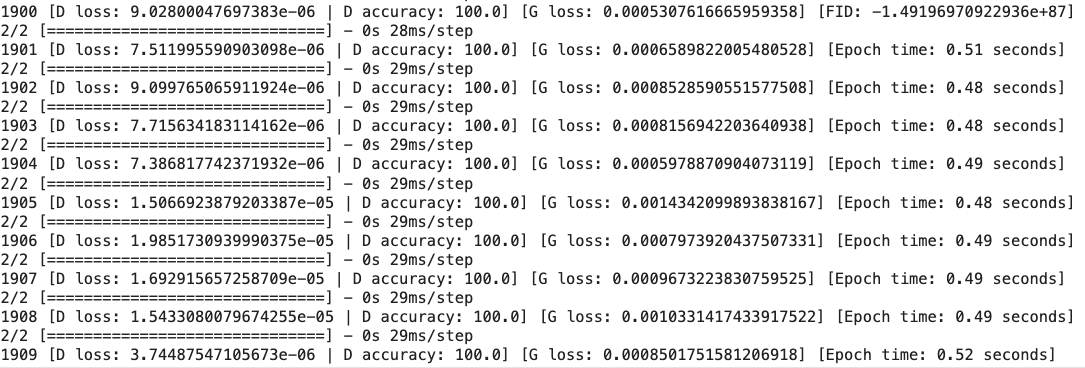
\includegraphics[width=1.2\linewidth]{./Images/model_accuracy.jpg}
    \caption{Training accuracy}
    \label{fig:my_picture}
\end{figure}

\begin{figure}[H]
    \centering
    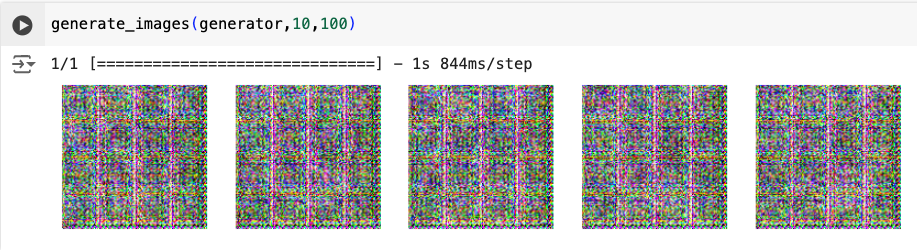
\includegraphics[width=1.2\linewidth]{./Images/generate_images.jpg}
    \caption{Generate images}
    \label{fig:my_picture}
\end{figure}


FID (Fréchet Inception Distance) quantifies the difference between generated data and real 
data by comparing their distribution in the Inception network feature space. FID takes into 
account the overall distribution of generated data and real data, and can reflect the quality 
and diversity of generated data. A low FID value indicates that the distribution of generated 
data is very close to the distribution of real data, that is, the generated data is both realistic 
and diverse, so FID is a more suitable indicator for evaluating the performance of generative models.

\newpage
\chapter{Experiments}
\label{Experiments}


\section*{Model select}
Approximately a decade has passed since Goodfellow introduced Generative Adversarial Networks (GANs), 
during which numerous variants of GAN models have been developed. For the purpose of this study, 
I have selected seven distinct GAN models for examination and minimal implementation: Standard GANs, 
Conditional GANs, Auxiliary Classifier GANs, Cycle GANs, Domain Transfer Network GANs, Coupled GANs, 
and Style GANs. The primary criterion for selection is training time, with only one model chosen for 
further in-depth analysis. Due to the extensive training time required, I ultimately selected Standard GANs for detailed study.


\section*{Model Structure}

In this step, I compared two types of standard GANs. The first model utilized dense layers, while the 
second model employed convolutional layers. The structure of the generator and discriminator was modified 
accordingly, while all other hyperparameters were kept constant. Both models were trained on the MNIST 
dataset for 1000 epochs. Upon comparing the generated images, it was observed that the GAN with the convolutional 
neural network (CNN) architecture outperformed the one with the dense layer architecture in terms of image quality. 
Consequently, I selected the standard GAN model implemented with convolutional layers for further experiments.

\begin{figure}[H]
    \centering
    \begin{subfigure}[b]{0.45\linewidth}
        \centering
        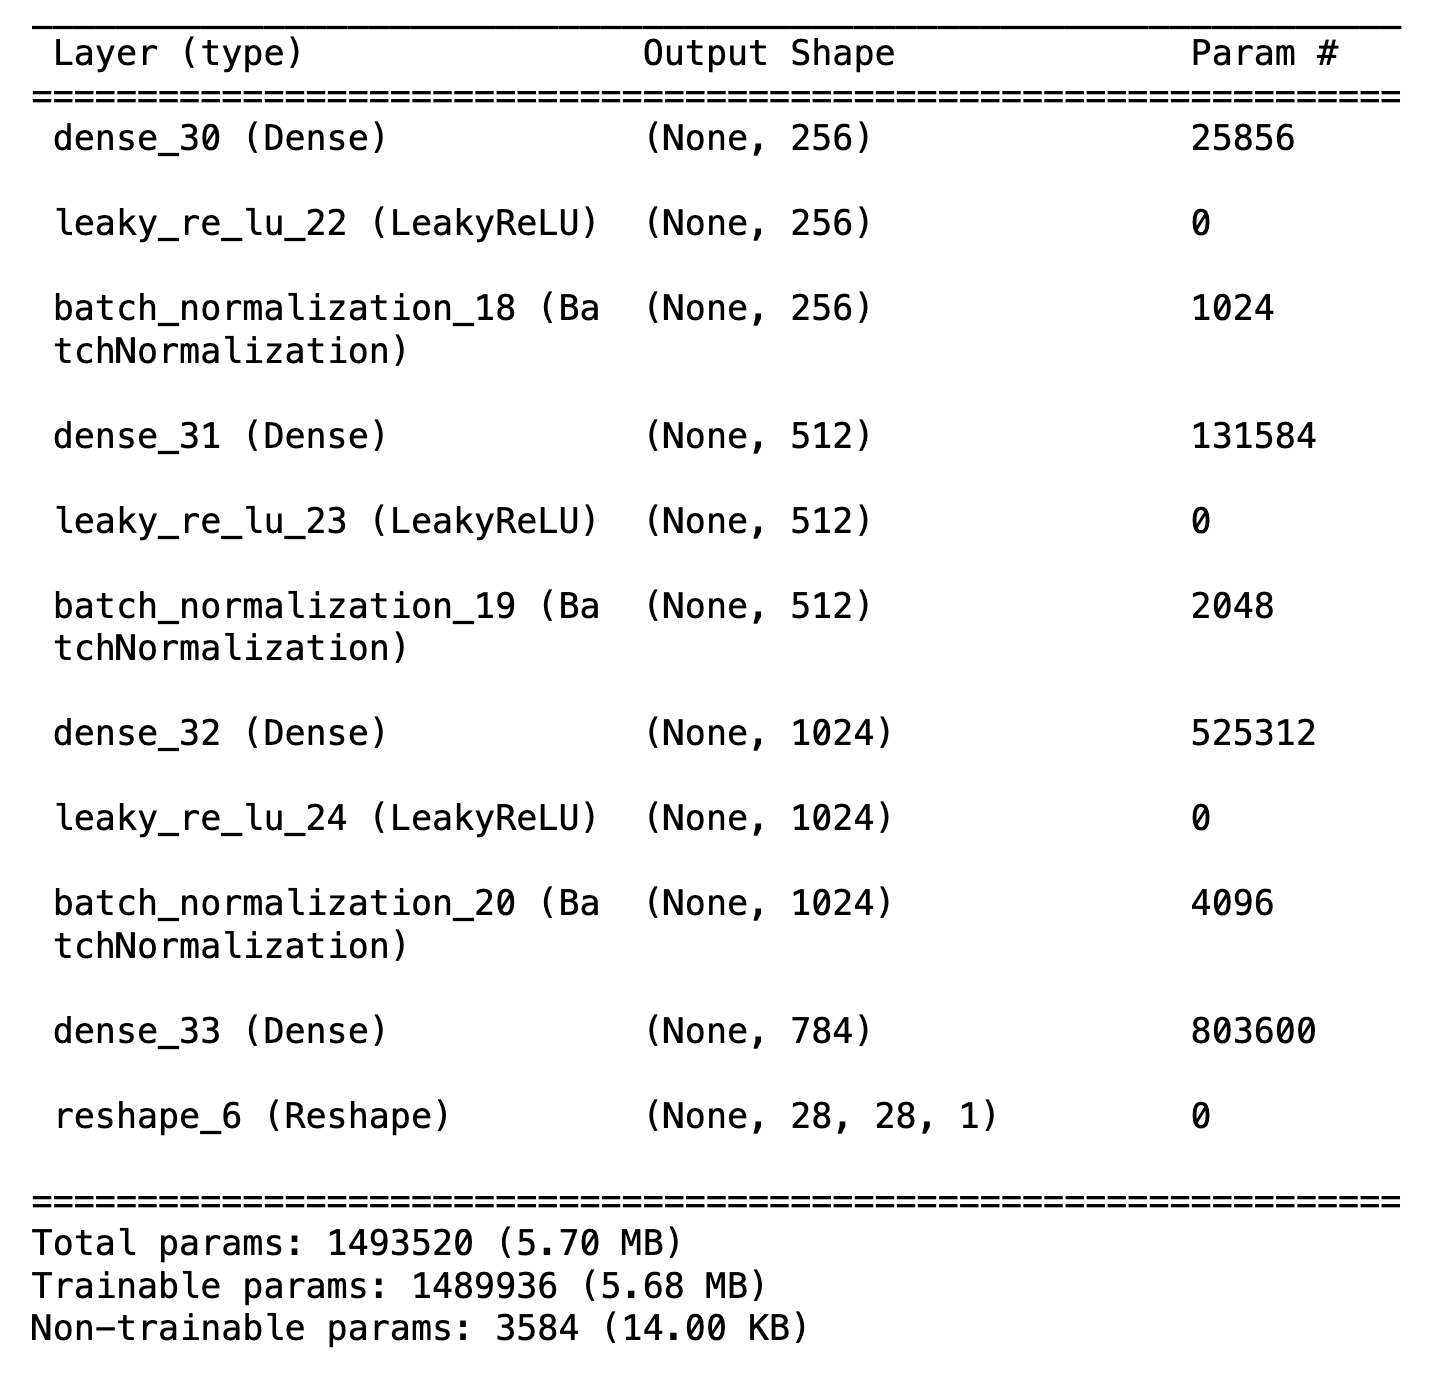
\includegraphics[width=\linewidth]{./Images/generator_dense.jpg}
        \caption{Generator with dense layer}
        \label{fig:Dense}
    \end{subfigure}
    \hspace{0.05\linewidth}
    \begin{subfigure}[b]{0.45\linewidth}
        \centering
        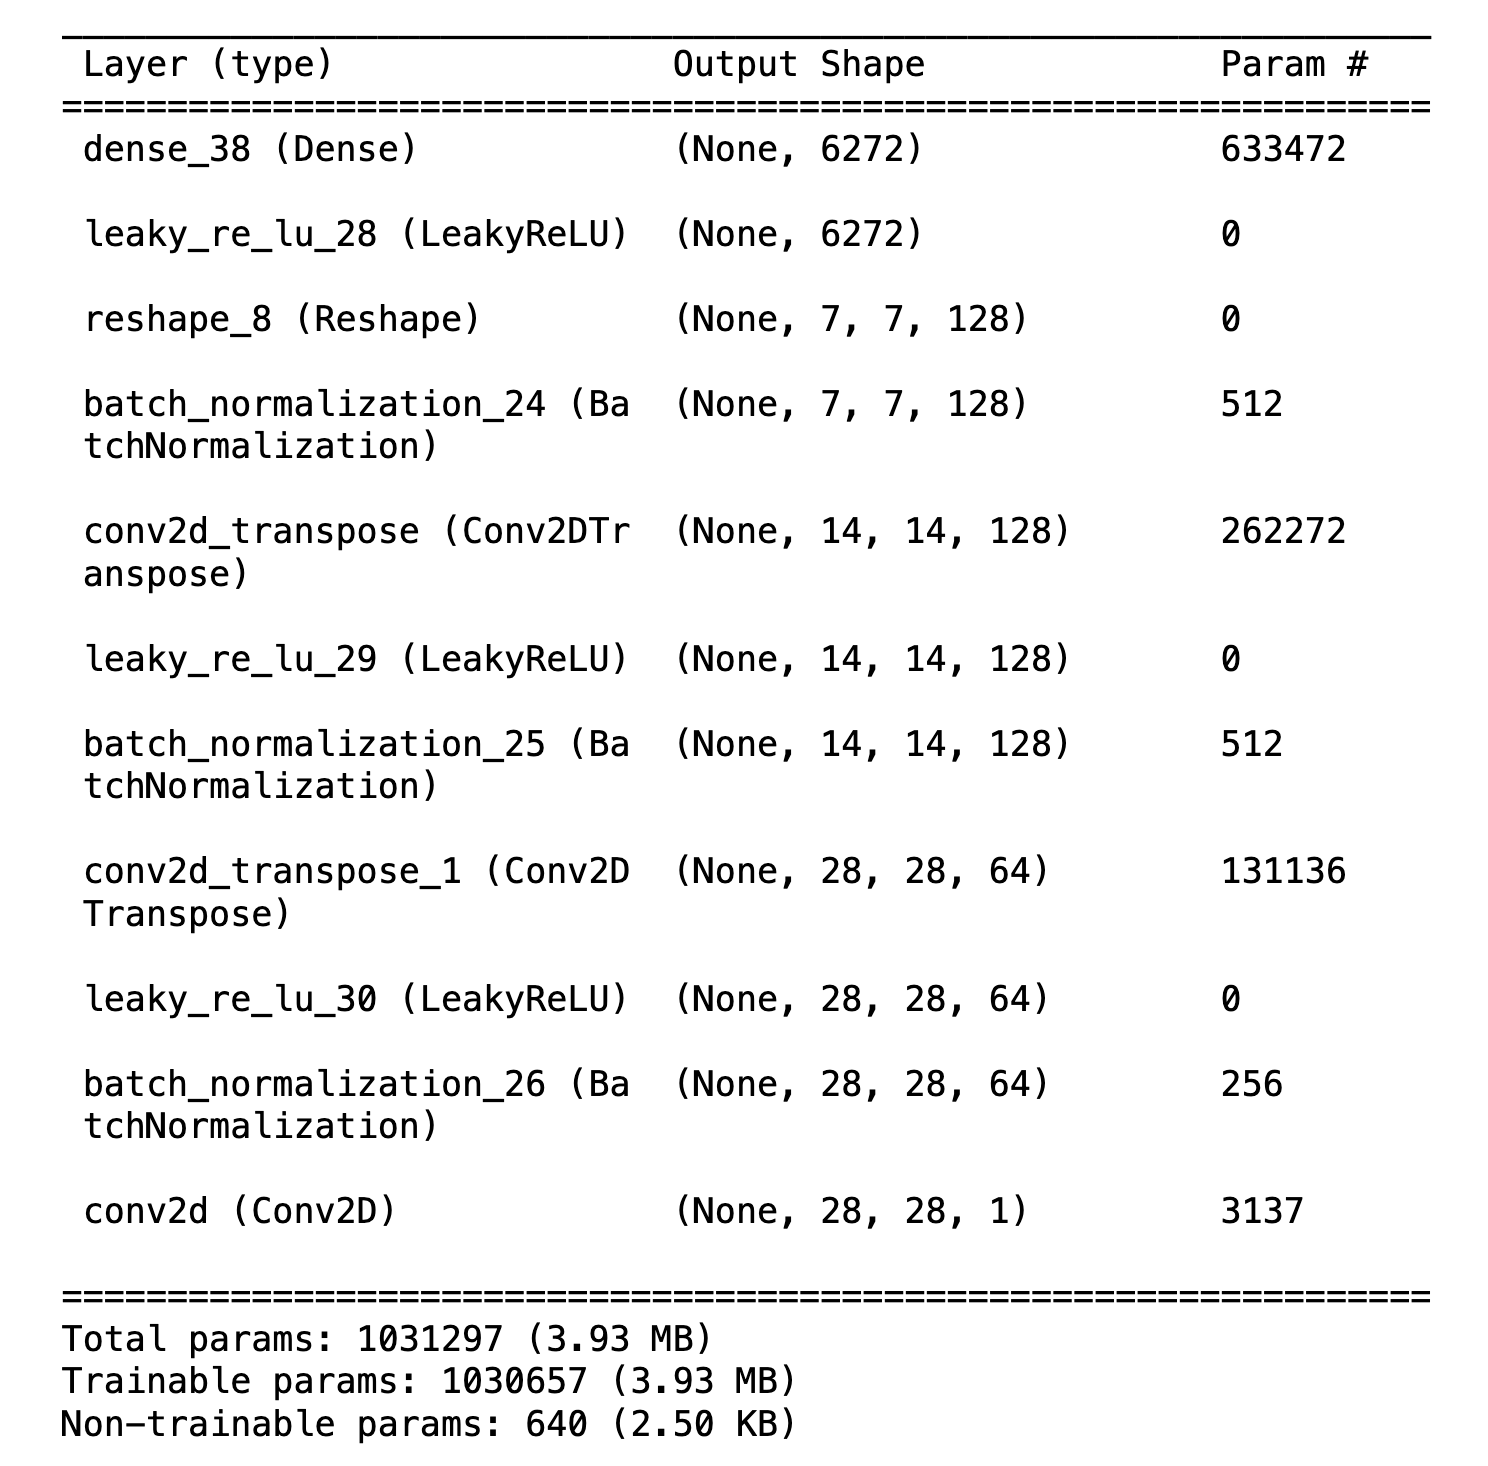
\includegraphics[width=\linewidth]{./Images/generator_cnn.jpg}
        \caption{Generator with convelution layer}
        \label{fig:Conv2D Transpose}
    \end{subfigure}
    \caption{The structure for generator}
    \label{fig:combined}
\end{figure}


\begin{figure}[H]
    \centering
    \begin{subfigure}[b]{0.45\linewidth}
        \centering
        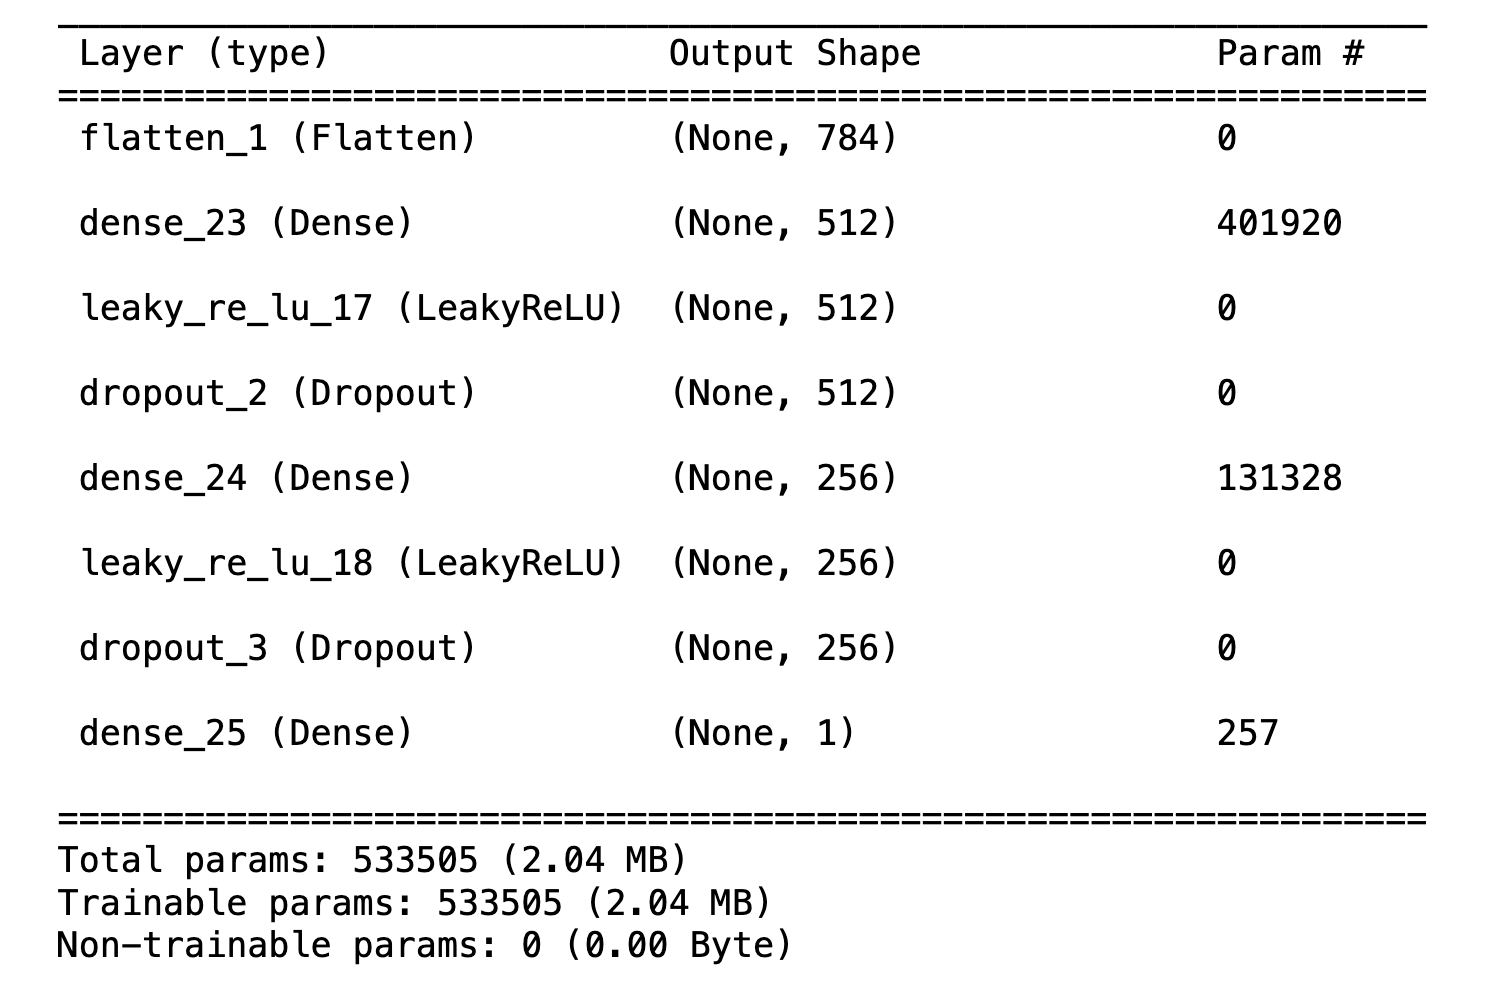
\includegraphics[width=\linewidth]{./Images/discriminator_dense.jpg}
        \caption{Discriminator with dense layer}
        \label{fig:Dense}
    \end{subfigure}
    \hspace{0.05\linewidth}
    \begin{subfigure}[b]{0.45\linewidth}
        \centering
        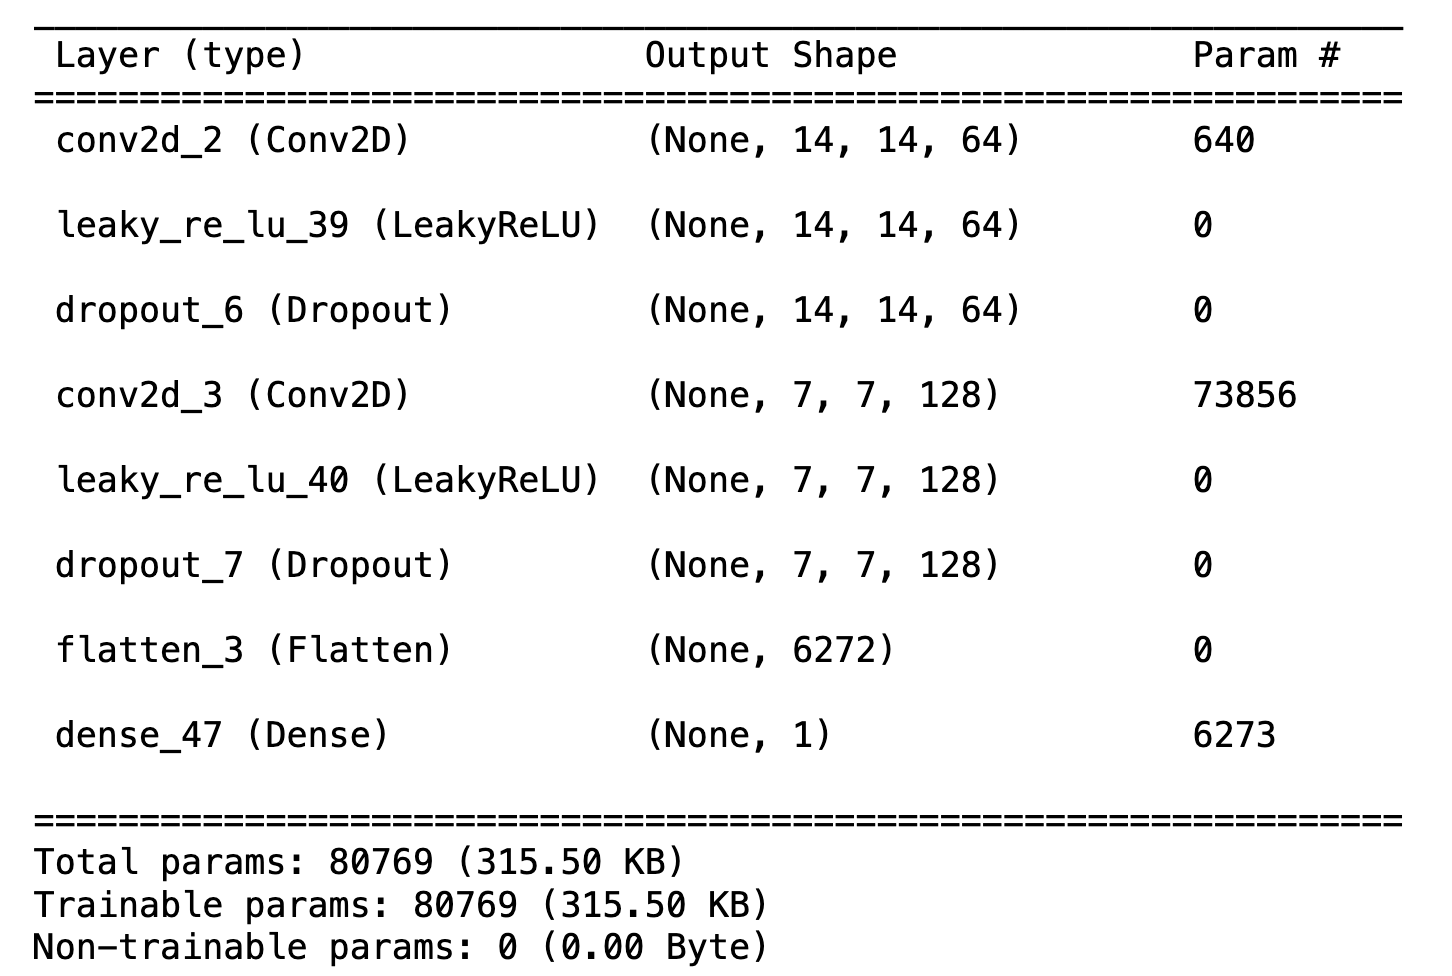
\includegraphics[width=\linewidth]{./Images/discriminator_cnn.jpg}
        \caption{Discriminator with convelution layer}
        \label{fig:Conv2D Transpose}
    \end{subfigure}
    \caption{The structure for discriminator}
    \label{fig:combined}
\end{figure}


\begin{figure}[H]
    \centering
    \begin{subfigure}[b]{\linewidth}
        \centering
        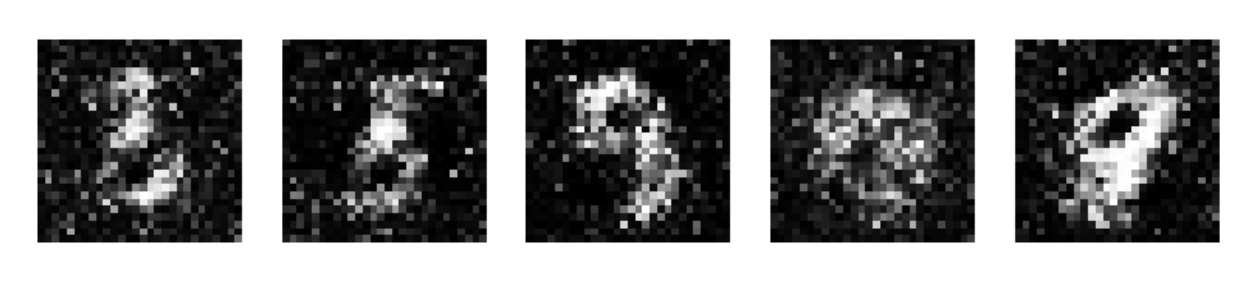
\includegraphics[width=0.7\linewidth]{./Images/generate_image_by_dense_layer.jpg}
        \caption{Images generate by dense structure}
        \label{fig:Dense}
    \end{subfigure}
    \vspace{0.05\linewidth} 
    \begin{subfigure}[b]{\linewidth}
        \centering
        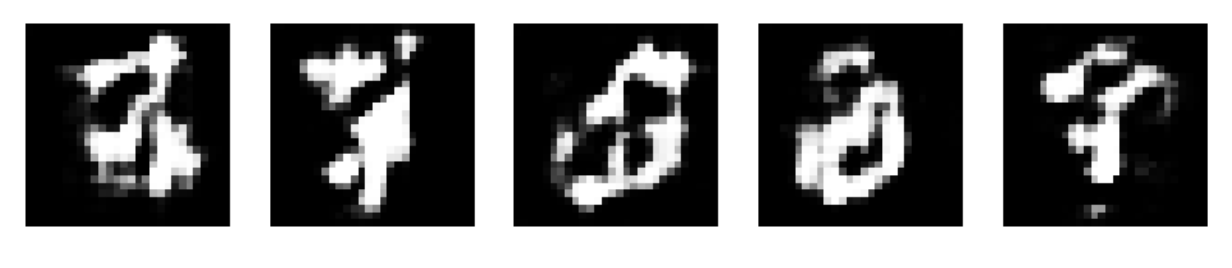
\includegraphics[width=0.7\linewidth]{./Images/generate_image_by_Convelution_layer.jpg}
        \caption{Images generate by convelution structure}
        \label{fig:Conv2DTranspose}
    \end{subfigure}
    \caption{Model performance 1000 epochs}
    \label{fig:combined}
\end{figure}








\section*{Data Augmentation}

I conducted three training runs of the standard GAN model, both with and without data augmentation, 
and compared the FID scores. The results indicate that data augmentation generally led to lower optimization performance.


\begin{figure}[H]
    \centering
    \begin{subfigure}[b]{\linewidth}
        \centering
        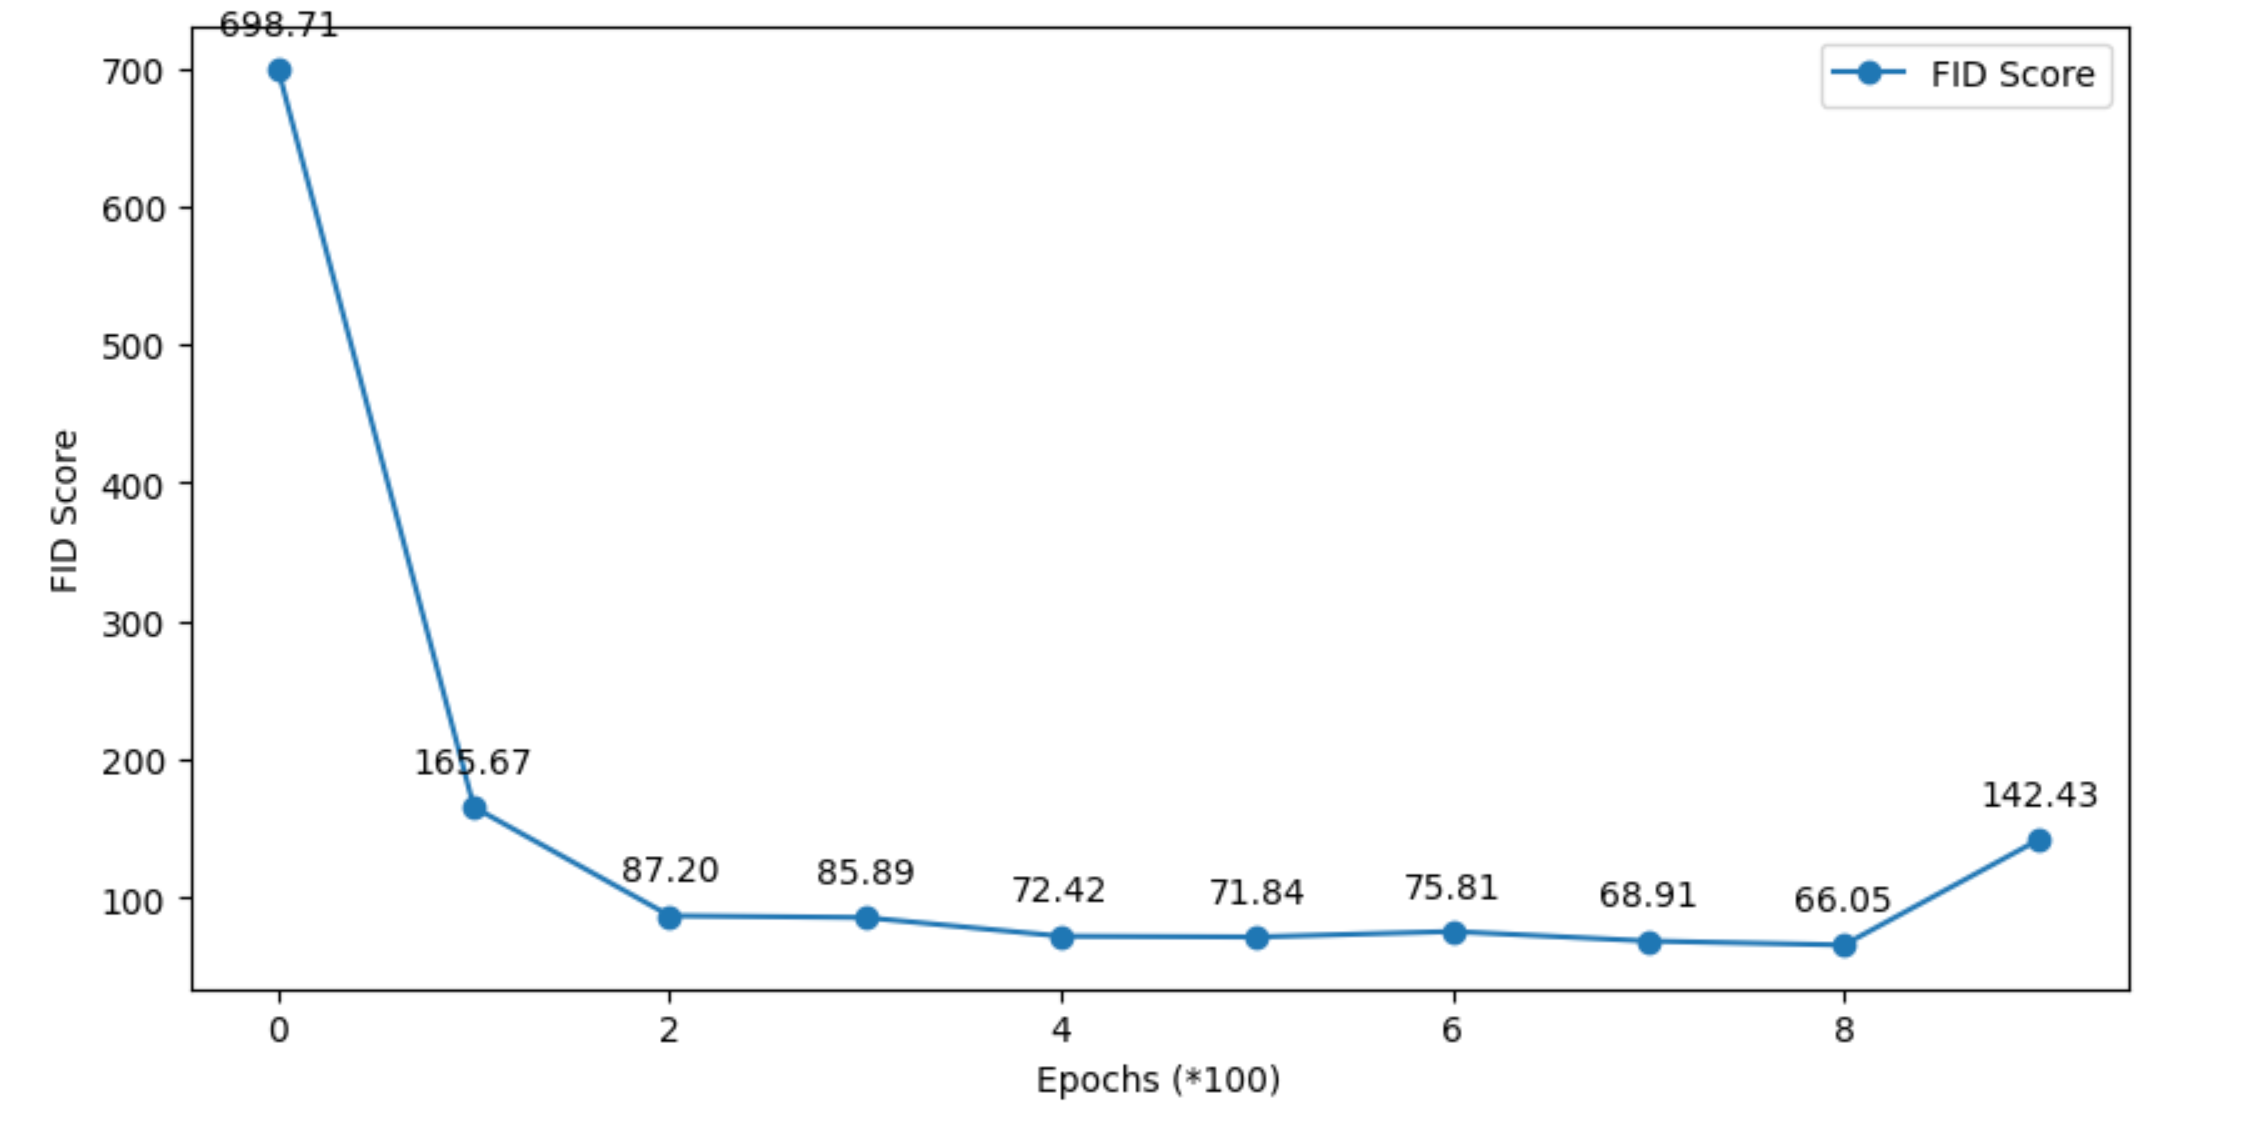
\includegraphics[width=0.8\linewidth]{./Images/standard_GAN_without_data_augementation1.jpg}
        \caption{Standard GAN without data augmentation 1}
        \label{fig:Dense}
    \end{subfigure}
    \vspace{0.05\linewidth} 
    \begin{subfigure}[b]{\linewidth}
        \centering
        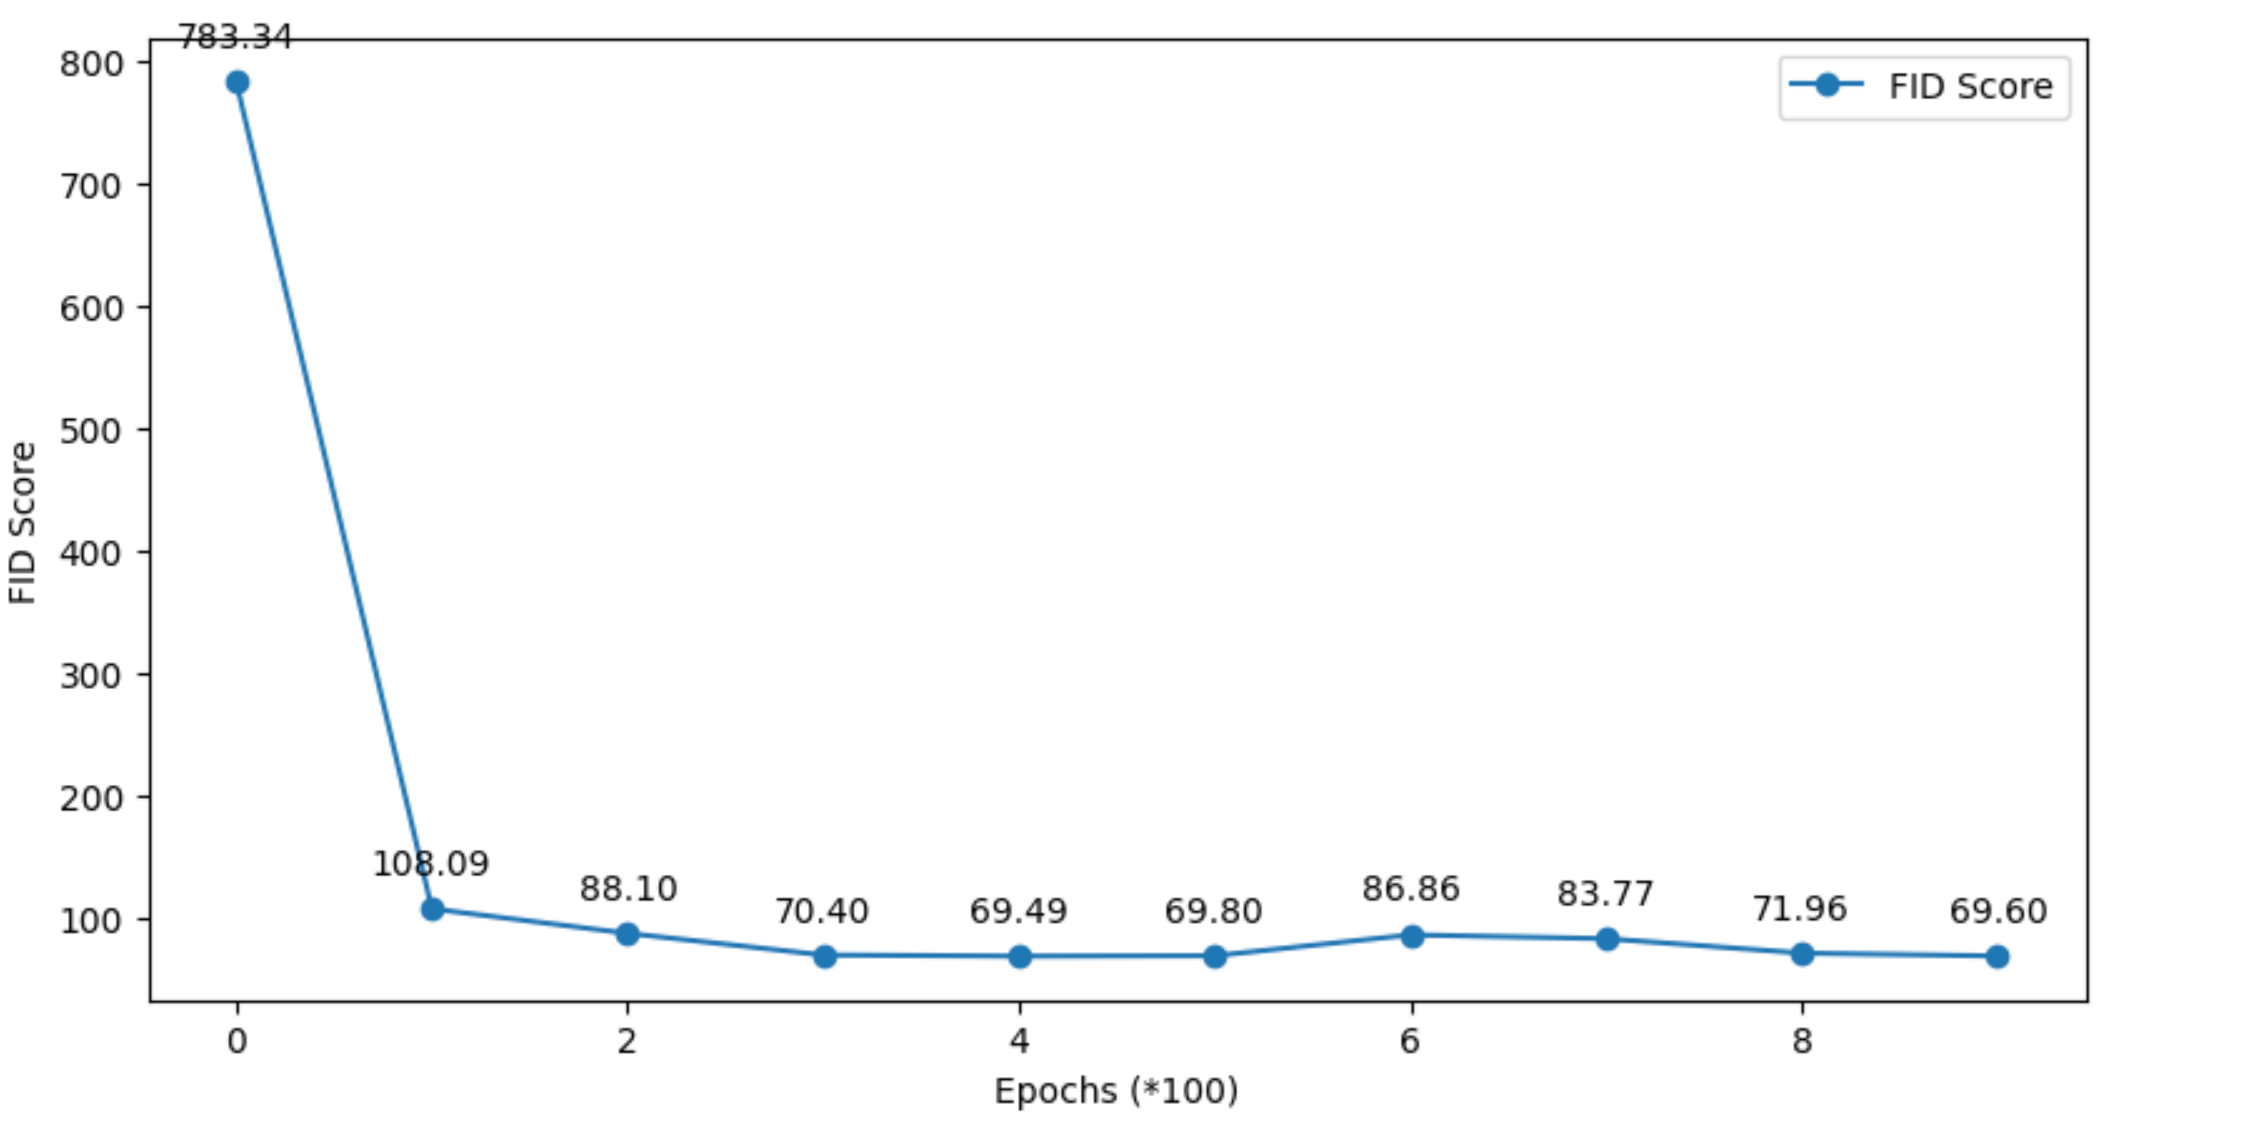
\includegraphics[width=0.8\linewidth]{./Images/standard_GAN_without_data_augementation2.jpg}
        \caption{Standard GAN without data augmentation 2}
        \label{fig:Conv2DTranspose}
    \end{subfigure}
    \begin{subfigure}[b]{\linewidth}
        \centering
        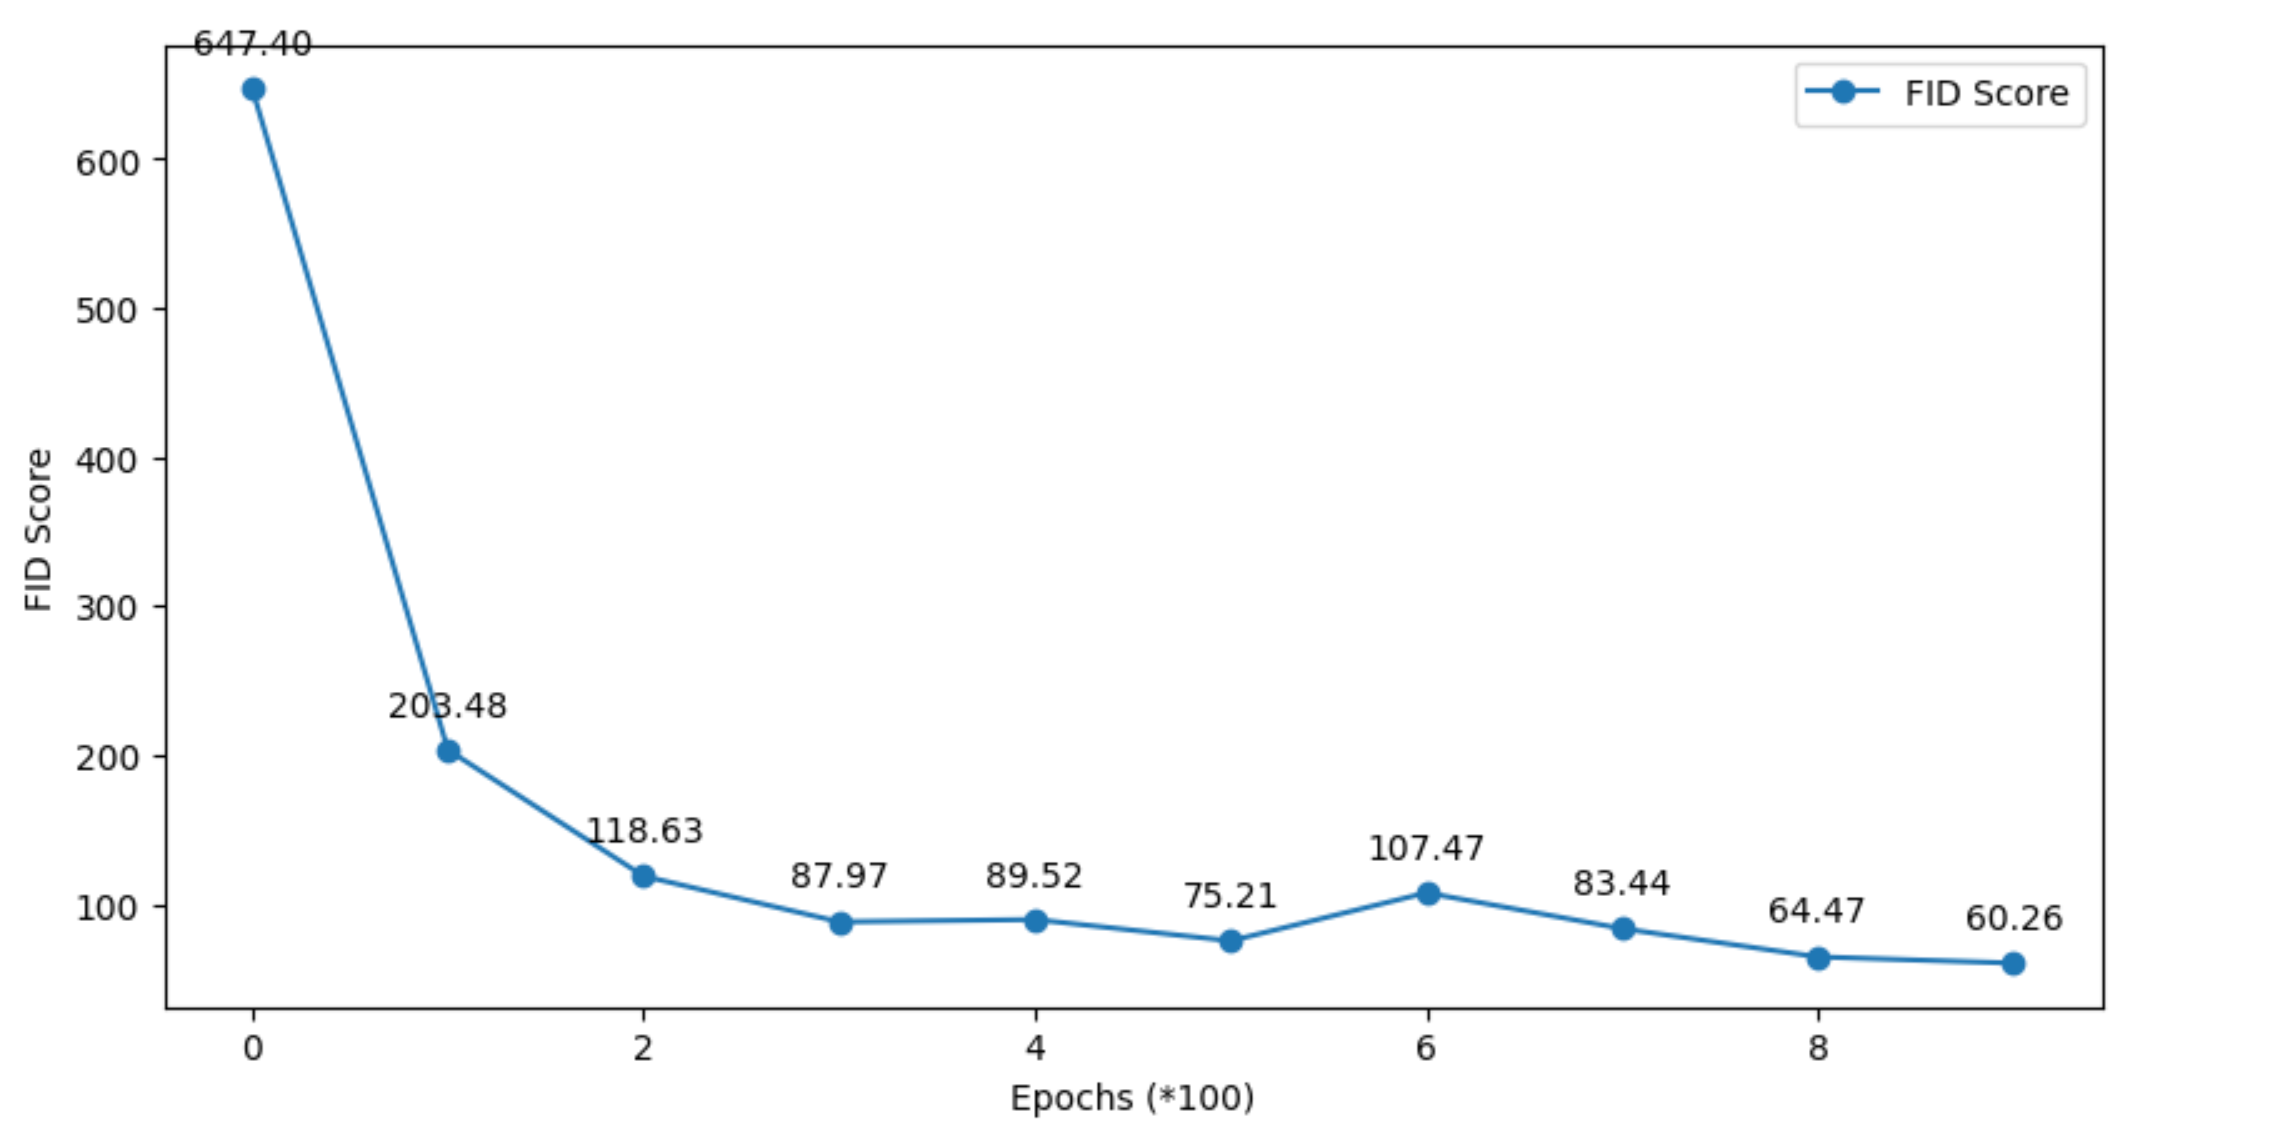
\includegraphics[width=0.8\linewidth]{./Images/standard_GAN_without_data_augementation3.jpg}
        \caption{Standard GAN without data augmentation 3}
        \label{fig:Conv2DTranspose}
    \end{subfigure}
    \caption{The FID scores for standard GAN without data augmentation}
    \label{fig:combined}
\end{figure}


\begin{figure}[H]
    \centering
    \begin{subfigure}[b]{\linewidth}
        \centering
        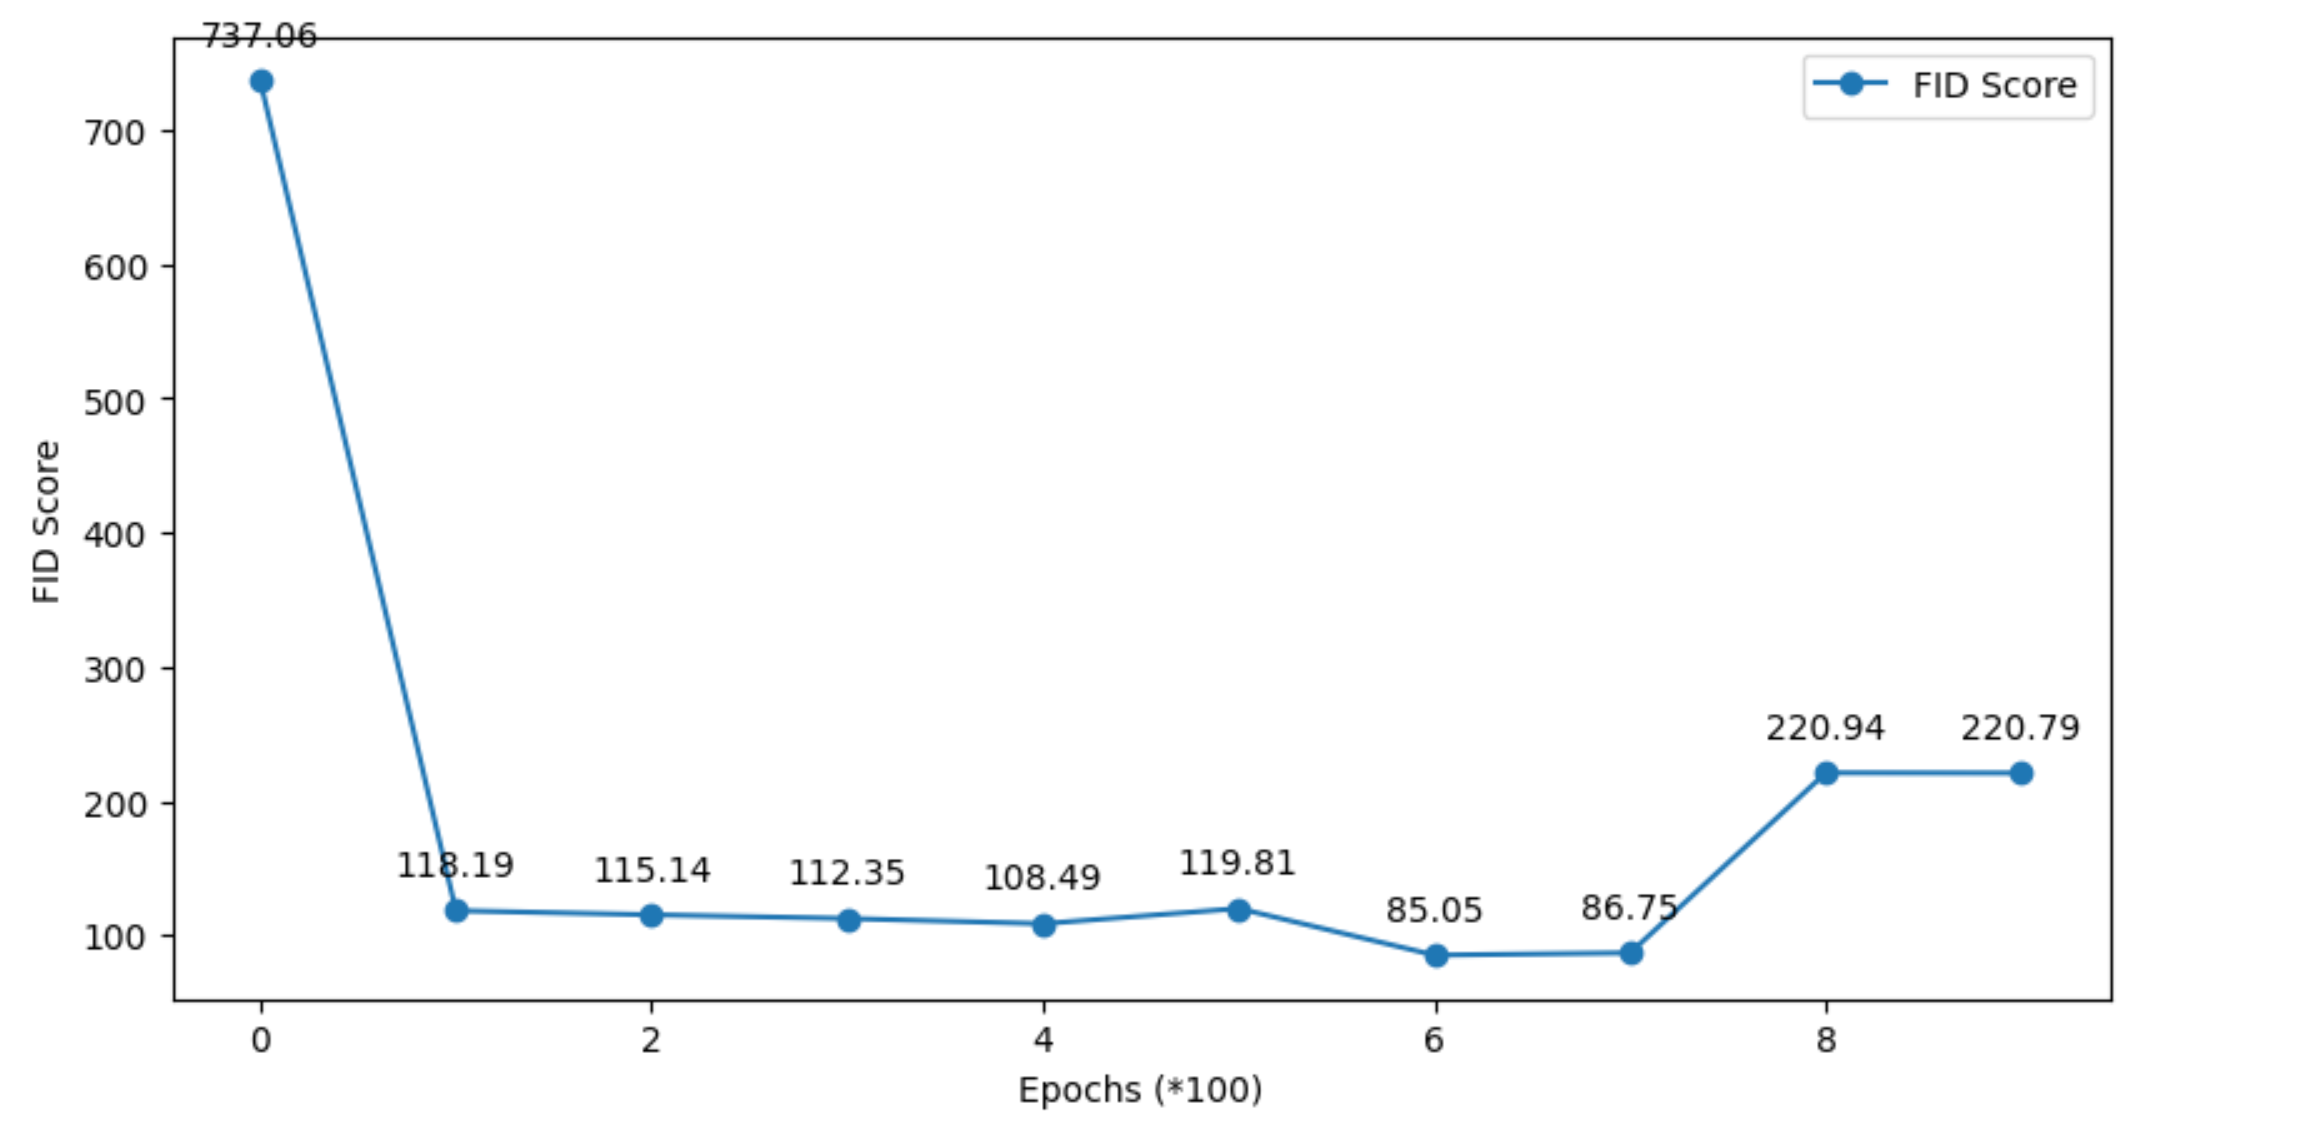
\includegraphics[width=0.84\linewidth]{./Images/standard_GAN_with_data_augementation1.jpg}
        \caption{Standard GAN with data augmentation 1}
        \label{fig:Dense}
    \end{subfigure}
    \vspace{0.05\linewidth} 
    \begin{subfigure}[b]{\linewidth}
        \centering
        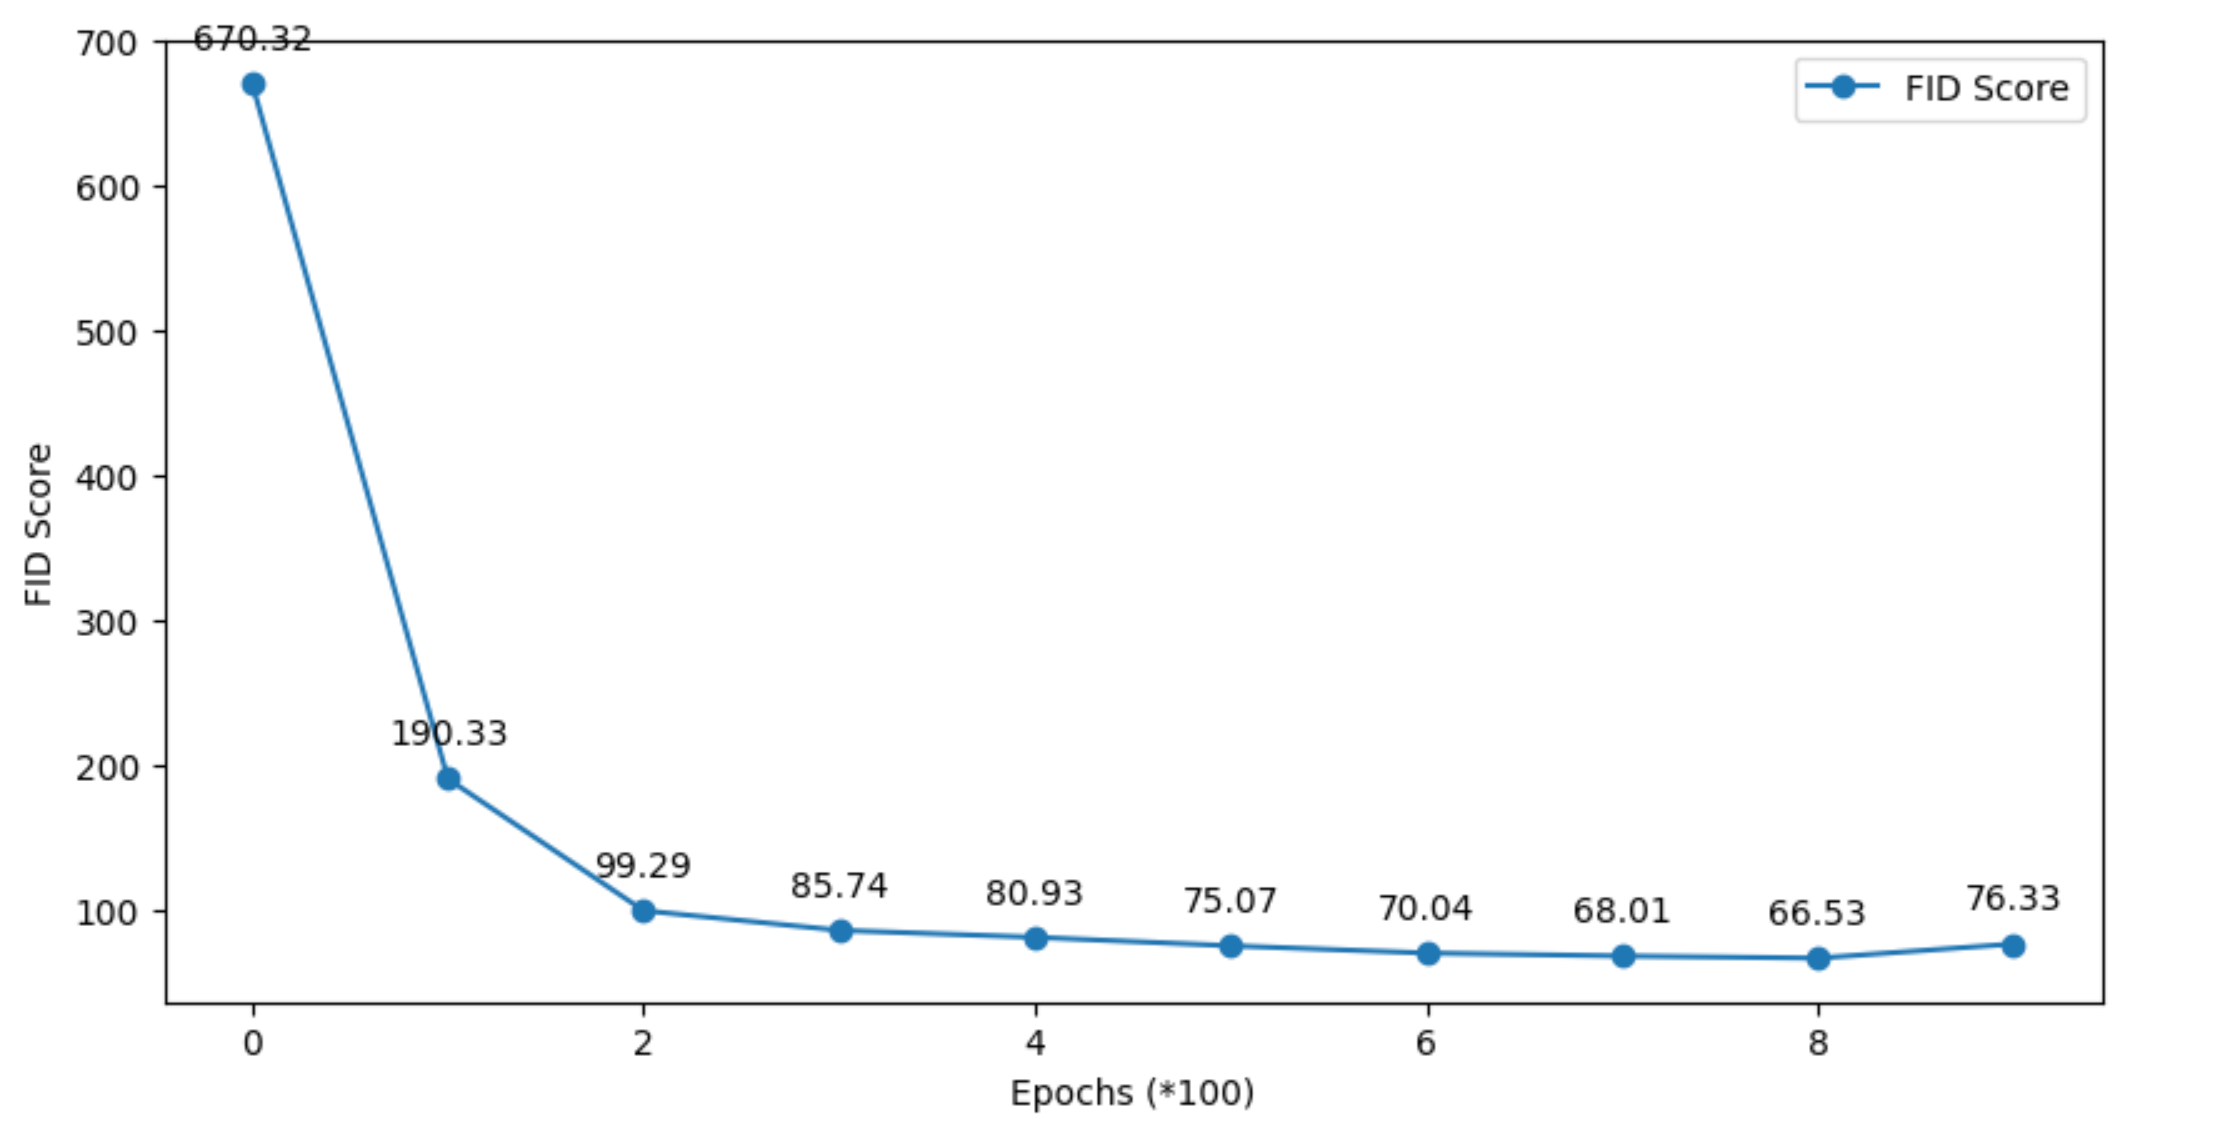
\includegraphics[width=0.8\linewidth]{./Images/standard_GAN_with_data_augementation2.jpg}
        \caption{Standard GAN with data augmentation 2}
        \label{fig:Conv2DTranspose}
    \end{subfigure}
    \begin{subfigure}[b]{\linewidth}
        \centering
        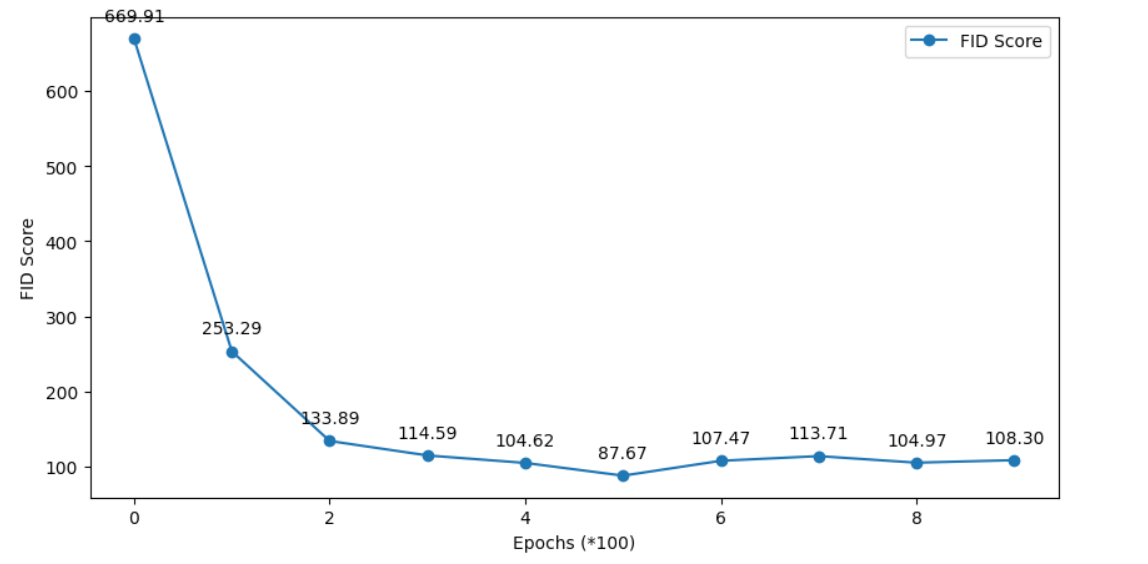
\includegraphics[width=0.8\linewidth]{./Images/standard_GAN_with_data_augementation3.jpg}
        \caption{Standard GAN with data augmentation 3}
        \label{fig:Conv2DTranspose}
    \end{subfigure}
    \caption{The FID scores for standard GAN with data augmentation}
    \label{fig:combined}
\end{figure}




\section*{Apply New Dataset}



\newpage
\chapter{Discussion}
\label{Discussion}

In this chapter I provide a discussion and concluding remarks...


\newpage
\appendix
\chapter{Appendix}
\label{Code}
\section*{Code}

% First code block
\begin{lstlisting}[style=mypython, caption=GAN model with dense layers]
import tensorflow as tf
from tensorflow.keras.layers import Dense, Reshape, Flatten, Dropout, LeakyReLU, BatchNormalization
from tensorflow.keras.models import Sequential
from tensorflow.keras.optimizers import Adam
from scipy.linalg import sqrtm
import numpy as np
import time
import matplotlib.pyplot as plt

np.random.seed(1000)
tf.random.set_seed(1000)

# input 100
# output 28*28*1

def build_generator():
    model = Sequential()
    
    # increase the dimension
    model.add(Dense(256, input_dim=100))
    model.add(LeakyReLU(alpha=0.2))
    model.add(BatchNormalization(momentum=0.8))
    
    model.add(Dense(512))
    model.add(LeakyReLU(alpha=0.2))
    model.add(BatchNormalization(momentum=0.8))
    
    model.add(Dense(1024))
    model.add(LeakyReLU(alpha=0.2))
    model.add(BatchNormalization(momentum=0.8))
    
    model.add(Dense(28*28, activation='tanh'))
    model.add(Reshape((28, 28, 1)))

    return model

# input 28*28*1
# output 1

def build_discriminator():
    model = Sequential()
    
    model.add(Flatten(input_shape=(28, 28, 1)))
    
    model.add(Dense(512))
    model.add(LeakyReLU(alpha=0.2))
    model.add(Dropout(0.25))
    
    model.add(Dense(256))
    model.add(LeakyReLU(alpha=0.2))
    model.add(Dropout(0.25))
    
    model.add(Dense(1, activation='sigmoid'))

    return model

# Load and preprocess the MNIST dataset
(x_train, _), (_, _) = tf.keras.datasets.mnist.load_data()
x_train = (x_train - 127.5) / 127.5
x_train = np.expand_dims(x_train, axis=3)

# Calculate FID function
def calculate_fid(real_images, fake_images):
    act1 = real_images.reshape((real_images.shape[0], -1))
    mu1, sigma1 = act1.mean(axis=0), np.cov(act1, rowvar=False)
    
    act2 = fake_images.reshape((fake_images.shape[0], -1))
    mu2, sigma2 = act2.mean(axis=0), np.cov(act2, rowvar=False)
    
    ssdiff = np.sum((mu1 - mu2)**2.0)
    covmean = sqrtm(sigma1.dot(sigma2))
    
    if np.iscomplexobj(covmean):
        covmean = covmean.real
    
    fid = ssdiff + np.trace(sigma1 + sigma2 - 2.0 * covmean)
    
    return fid

def train_gan(epochs=1000, batch_size=64, p_epoch=100):
    generator = build_generator()
    discriminator = build_discriminator()

    discriminator.compile(loss='binary_crossentropy', optimizer=Adam(0.0002, 0.5), metrics=['accuracy'])
    discriminator.trainable = False

    gan_input = tf.keras.Input(shape=(100,))
    gan_output = discriminator(generator(gan_input))
    gan = tf.keras.Model(gan_input, gan_output)
    gan.compile(loss='binary_crossentropy', optimizer=Adam(0.0002, 0.5))

    half_batch = int(batch_size / 2)
    
    d_losses = []
    g_losses = []
    d_acc = []
    fid_scores = []  # List to store FID scores
    
    start_time = time.time()  # Record the start time

    for epoch in range(epochs):
        # Select a random half batch of real images
        idx = np.random.randint(0, x_train.shape[0], half_batch)
        real_images = x_train[idx]

        # Generate a half batch of new fake images
        noise = np.random.normal(0, 1, (half_batch, 100))
        fake_images = generator.predict(noise)

        # Train the discriminator
        real_labels = np.ones((half_batch, 1))
        fake_labels = np.zeros((half_batch, 1))

        d_loss_real = discriminator.train_on_batch(real_images, real_labels)
        d_loss_fake = discriminator.train_on_batch(fake_images, fake_labels)
        d_loss = 0.5 * np.add(d_loss_real, d_loss_fake)

        # Train the generator
        noise = np.random.normal(0, 1, (batch_size, 100))
        valid_y = np.ones((batch_size, 1))

        g_loss = gan.train_on_batch(noise, valid_y)

        # Record the losses
        d_losses.append(d_loss[0])
        g_losses.append(g_loss)
        d_acc.append(d_loss[1] * 100)
        
        # Calculate and print FID every p_epoch epochs
        if epoch % p_epoch == 0:
            noise = np.random.normal(0, 1, (1000, 100))
            fake_images = generator.predict(noise)
            fid = calculate_fid(x_train[:1000], fake_images)
            fid_scores.append(fid)
            print(f"{epoch} [D loss: {d_loss[0]}, acc.: {100 * d_loss[1]}%] [G loss: {g_loss}] [FID: {fid}]")

    end_time = time.time()  # Record the end time
    total_time = end_time - start_time
    print(f"Total training time: {total_time:.2f} seconds")
    return generator, d_losses, g_losses, d_acc, fid_scores
\end{lstlisting}




\begin{lstlisting}[style=mypython, caption=GAN model with Convolutional layers]
    import tensorflow as tf
    from tensorflow.keras.layers import Dense, Reshape, Flatten, Dropout, LeakyReLU, Conv2D, Conv2DTranspose, BatchNormalization
    from tensorflow.keras.models import Sequential
    from tensorflow.keras.optimizers import Adam
    from scipy.linalg import sqrtm
    import numpy as np
    import time
    import matplotlib.pyplot as plt
    
    np.random.seed(1000)
    tf.random.set_seed(1000)
    
    # input 100
    # output 28*28*1
    
    def build_generator():
        model = Sequential()
        
        # increase the dimension
        model.add(Dense(7*7*128, input_dim=100))
        model.add(LeakyReLU(alpha=0.2))
        model.add(Reshape((7, 7, 128)))
        model.add(BatchNormalization(momentum=0.8))
    
        model.add(Conv2DTranspose(128, kernel_size=4, strides=2, padding='same'))
        model.add(LeakyReLU(alpha=0.2))
        model.add(BatchNormalization(momentum=0.8))
    
        model.add(Conv2DTranspose(64, kernel_size=4, strides=2, padding='same'))
        model.add(LeakyReLU(alpha=0.2))
        model.add(BatchNormalization(momentum=0.8))
    
        model.add(Conv2D(1, kernel_size=7, activation='tanh', padding='same'))
    
        return model
    
    # input 28*28*1
    # output 1
    
    def build_discriminator():
        model = Sequential()
        
        model.add(Conv2D(64, kernel_size=3, strides=2, input_shape=(28, 28, 1), padding='same'))
        model.add(LeakyReLU(alpha=0.2))
        model.add(Dropout(0.25))
    
        model.add(Conv2D(128, kernel_size=3, strides=2, padding='same'))
        model.add(LeakyReLU(alpha=0.2))
        model.add(Dropout(0.25))
    
        model.add(Flatten())
        model.add(Dense(1, activation='sigmoid'))
    
        return model
    
    # Load and preprocess the MNIST dataset
    (x_train, _), (_, _) = tf.keras.datasets.mnist.load_data()
    x_train = (x_train - 127.5) / 127.5
    x_train = np.expand_dims(x_train, axis=3)
    
    # Calculate FID function
    def calculate_fid(real_images, fake_images):
        act1 = real_images.reshape((real_images.shape[0], -1))
        mu1, sigma1 = act1.mean(axis=0), np.cov(act1, rowvar=False)
        
        act2 = fake_images.reshape((fake_images.shape[0], -1))
        mu2, sigma2 = act2.mean(axis=0), np.cov(act2, rowvar=False)
        
        ssdiff = np.sum((mu1 - mu2)**2.0)
        covmean = sqrtm(sigma1.dot(sigma2))
        
        if np.iscomplexobj(covmean):
            covmean = covmean.real
        
        fid = ssdiff + np.trace(sigma1 + sigma2 - 2.0 * covmean)
        
        return fid
    
    def train_gan(epochs=1000, batch_size=64, p_epoch=100):
        generator = build_generator()
        discriminator = build_discriminator()
    
        discriminator.compile(loss='binary_crossentropy', optimizer=Adam(0.0002, 0.5), metrics=['accuracy'])
        discriminator.trainable = False
    
        gan_input = tf.keras.Input(shape=(100,))
        gan_output = discriminator(generator(gan_input))
        gan = tf.keras.Model(gan_input, gan_output)
        gan.compile(loss='binary_crossentropy', optimizer=Adam(0.0002, 0.5))
    
        # using half batches for the discriminator ensures balanced and efficient training, 
        # better memory management, and more stable training dynamics in GANs.
        half_batch = int(batch_size / 2)
        
        d_losses = []
        g_losses = []
        d_acc = []
        fid_scores = []  # List to store FID scores
        
        start_time = time.time()  # Record the start time
    
        for epoch in range(epochs):
            # Select a random half batch of real images
            idx = np.random.randint(0, x_train.shape[0], half_batch)
            real_images = x_train[idx]
    
            # Generate a half batch of new fake images
            noise = np.random.normal(0, 1, (half_batch, 100))
            fake_images = generator.predict(noise)
    
            # Train the discriminator
            real_labels = np.ones((half_batch, 1))
            fake_labels = np.zeros((half_batch, 1))
    
            d_loss_real = discriminator.train_on_batch(real_images, real_labels)
            d_loss_fake = discriminator.train_on_batch(fake_images, fake_labels)
            d_loss = 0.5 * np.add(d_loss_real, d_loss_fake)
    
            # Train the generator
            noise = np.random.normal(0, 1, (batch_size, 100))
            valid_y = np.ones((batch_size, 1))
    
            g_loss = gan.train_on_batch(noise, valid_y)
    
            # Record the losses
            d_losses.append(d_loss[0])
            g_losses.append(g_loss)
            d_acc.append(d_loss[1] * 100)
            
            # Calculate FID every p_epoch epochs
            if epoch % p_epoch == 0:
                noise = np.random.normal(0, 1, (1000, 100))
                fake_images = generator.predict(noise)
                fid = calculate_fid(x_train[:1000], fake_images)
                fid_scores.append(fid)
                print(f"{epoch} [D loss: {d_loss[0]}, acc.: {100 * d_loss[1]}%] [G loss: {g_loss}] [FID: {fid}]")
        
        end_time = time.time()  # Record the end time
        total_time = end_time - start_time
        print(f"Total training time: {total_time:.2f} seconds")
        return generator, d_losses, g_losses, d_acc, fid_scores
\end{lstlisting}


\begin{lstlisting}[style=mypython, caption= Explore data augmentaion 1]
    import tensorflow as tf
    from tensorflow.keras.layers import Dense, Reshape, Flatten, Dropout, LeakyReLU, Conv2D, Conv2DTranspose, BatchNormalization
    from tensorflow.keras.models import Sequential
    from tensorflow.keras.optimizers import Adam
    from scipy.linalg import sqrtm
    import numpy as np
    import time
    import matplotlib.pyplot as plt
    
    np.random.seed(1000)
    tf.random.set_seed(1000)
    
    # input 100
    # output 28*28*1
    
    def build_generator():
        model = Sequential()
        
        # increase the dimension
        model.add(Dense(7*7*128, input_dim=100))
        model.add(LeakyReLU(alpha=0.2))
        model.add(Reshape((7, 7, 128)))
        model.add(BatchNormalization(momentum=0.8))
    
        model.add(Conv2DTranspose(128, kernel_size=4, strides=2, padding='same'))
        model.add(LeakyReLU(alpha=0.2))
        model.add(BatchNormalization(momentum=0.8))
    
        model.add(Conv2DTranspose(64, kernel_size=4, strides=2, padding='same'))
        model.add(LeakyReLU(alpha=0.2))
        model.add(BatchNormalization(momentum=0.8))
    
        model.add(Conv2D(1, kernel_size=7, activation='tanh', padding='same'))
    
        return model
    
    # input 28*28*1
    # output 1
    
    def build_discriminator():
        model = Sequential()
        
        model.add(Conv2D(64, kernel_size=3, strides=2, input_shape=(28, 28, 1), padding='same'))
        model.add(LeakyReLU(alpha=0.2))
        model.add(Dropout(0.25))
    
        model.add(Conv2D(128, kernel_size=3, strides=2, padding='same'))
        model.add(LeakyReLU(alpha=0.2))
        model.add(Dropout(0.25))
    
        model.add(Flatten())
        model.add(Dense(1, activation='sigmoid'))
    
        return model
    
    (x_train, _), (_, _) = tf.keras.datasets.mnist.load_data()
    x_train = (x_train - 127.5) / 127.5
    x_train = np.expand_dims(x_train, axis=3)
    
    datagen = tf.keras.preprocessing.image.ImageDataGenerator(
        rotation_range=10,
        width_shift_range=0.1,
        height_shift_range=0.1,
        horizontal_flip=True
    )
    
    def calculate_fid(real_images, fake_images):
        act1 = real_images.reshape((real_images.shape[0], -1))
        mu1, sigma1 = act1.mean(axis=0), np.cov(act1, rowvar=False)
        
        act2 = fake_images.reshape((fake_images.shape[0], -1))
        mu2, sigma2 = act2.mean(axis=0), np.cov(act2, rowvar=False)
        
        ssdiff = np.sum((mu1 - mu2)**2.0)
        covmean = sqrtm(sigma1.dot(sigma2))
        
        if np.iscomplexobj(covmean):
            covmean = covmean.real
        
        fid = ssdiff + np.trace(sigma1 + sigma2 - 2.0 * covmean)
        
        return fid
    
    def train_gan(epochs=1000, batch_size=64, p_epoch=100):
        generator = build_generator()
        discriminator = build_discriminator()
    
        discriminator.compile(loss='binary_crossentropy', optimizer=Adam(0.0002, 0.5), metrics=['accuracy'])
        discriminator.trainable = False
    
        gan_input = tf.keras.Input(shape=(100,))
        gan_output = discriminator(generator(gan_input))
        gan = tf.keras.Model(gan_input, gan_output)
        gan.compile(loss='binary_crossentropy', optimizer=Adam(0.0002, 0.5))
    
        half_batch = int(batch_size / 2)
        
        d_losses = []
        g_losses = []
        d_acc = []
        fid_scores = []
        
        start_time = time.time()  # Record the start time
    
        for epoch in range(epochs):
            # Select a random half batch of real images
            idx = np.random.randint(0, x_train.shape[0], half_batch)
            real_images = x_train[idx]
    
            real_images_augmented = next(datagen.flow(real_images, batch_size=half_batch))
    
            # Generate a half batch of new fake images
            noise = np.random.normal(0, 1, (half_batch, 100))
            fake_images = generator.predict(noise)
    
            # Train the discriminator
            real_labels = np.ones((half_batch, 1))
            fake_labels = np.zeros((half_batch, 1))
    
            d_loss_real = discriminator.train_on_batch(real_images_augmented, real_labels)
            d_loss_fake = discriminator.train_on_batch(fake_images, fake_labels)
            d_loss = 0.5 * np.add(d_loss_real, d_loss_fake)
    
            # Train the generator
            noise = np.random.normal(0, 1, (batch_size, 100))
            valid_y = np.ones((batch_size, 1))
    
            g_loss = gan.train_on_batch(noise, valid_y)
    
            # Record the losses
            d_losses.append(d_loss[0])
            g_losses.append(g_loss)
            d_acc.append(d_loss[1] * 100)
            
            # Calculate FID every p_epoch epochs
            if epoch % p_epoch == 0:
                noise = np.random.normal(0, 1, (1000, 100))
                fake_images = generator.predict(noise)
                fid = calculate_fid(x_train[:1000], fake_images)
                fid_scores.append(fid)
                print(f"{epoch} [D loss: {d_loss[0]}, acc.: {100 * d_loss[1]}%] [G loss: {g_loss}] [FID: {fid}]")
    
        end_time = time.time()  # Record the end time
        total_time = end_time - start_time
        print(f"Total training time: {total_time:.2f} seconds")
        return generator, d_losses, g_losses, d_acc, fid_scores
    
    # Training the GAN with data augmentation and FID calculation
    generator, d_losses, g_losses, d_acc, fid_scores = train_gan(epochs=1000, batch_size=64, p_epoch=100)
\end{lstlisting}


\begin{lstlisting}[style=mypython, caption=Explore data augmentation 2]
    import tensorflow as tf
    from tensorflow.keras.layers import Dense, Reshape, Flatten, Dropout, LeakyReLU, Conv2D, Conv2DTranspose, BatchNormalization
    from tensorflow.keras.models import Sequential
    from tensorflow.keras.optimizers import Adam
    from scipy.linalg import sqrtm
    import numpy as np
    import time
    import matplotlib.pyplot as plt
    
    np.random.seed(1000)
    tf.random.set_seed(1000)
    
    # input 100
    # output 28*28*1
    
    def build_generator():
        model = Sequential()
        
        # increase the dimension
        model.add(Dense(7*7*128, input_dim=100))
        model.add(LeakyReLU(alpha=0.2))
        model.add(Reshape((7, 7, 128)))
        model.add(BatchNormalization(momentum=0.8))
    
        model.add(Conv2DTranspose(128, kernel_size=4, strides=2, padding='same'))
        model.add(LeakyReLU(alpha=0.2))
        model.add(BatchNormalization(momentum=0.8))
    
        model.add(Conv2DTranspose(64, kernel_size=4, strides=2, padding='same'))
        model.add(LeakyReLU(alpha=0.2))
        model.add(BatchNormalization(momentum=0.8))
    
        model.add(Conv2D(1, kernel_size=7, activation='tanh', padding='same'))
    
        return model
    
    # input 28*28*1
    # output 1
    
    def build_discriminator():
        model = Sequential()
        
        model.add(Conv2D(64, kernel_size=3, strides=2, input_shape=(28, 28, 1), padding='same'))
        model.add(LeakyReLU(alpha=0.2))
        model.add(Dropout(0.25))
    
        model.add(Conv2D(128, kernel_size=3, strides=2, padding='same'))
        model.add(LeakyReLU(alpha=0.2))
        model.add(Dropout(0.25))
    
        model.add(Flatten())
        model.add(Dense(1, activation='sigmoid'))
    
        return model
    
    (x_train, _), (_, _) = tf.keras.datasets.mnist.load_data()
    x_train = (x_train - 127.5) / 127.5
    x_train = np.expand_dims(x_train, axis=3)
    
    datagen = tf.keras.preprocessing.image.ImageDataGenerator(
        rotation_range=10,
        width_shift_range=0.1,
        height_shift_range=0.1,
    )
    
    def calculate_fid(real_images, fake_images):
        act1 = real_images.reshape((real_images.shape[0], -1))
        mu1, sigma1 = act1.mean(axis=0), np.cov(act1, rowvar=False)
        
        act2 = fake_images.reshape((fake_images.shape[0], -1))
        mu2, sigma2 = act2.mean(axis=0), np.cov(act2, rowvar=False)
        
        ssdiff = np.sum((mu1 - mu2)**2.0)
        covmean = sqrtm(sigma1.dot(sigma2))
        
        if np.iscomplexobj(covmean):
            covmean = covmean.real
        
        fid = ssdiff + np.trace(sigma1 + sigma2 - 2.0 * covmean)
        
        return fid
    
    def train_gan(epochs=1000, batch_size=64, p_epoch=100):
        generator = build_generator()
        discriminator = build_discriminator()
    
        discriminator.compile(loss='binary_crossentropy', optimizer=Adam(0.0002, 0.5), metrics=['accuracy'])
        discriminator.trainable = False
    
        gan_input = tf.keras.Input(shape=(100,))
        gan_output = discriminator(generator(gan_input))
        gan = tf.keras.Model(gan_input, gan_output)
        gan.compile(loss='binary_crossentropy', optimizer=Adam(0.0002, 0.5))
    
        half_batch = int(batch_size / 2)
        
        d_losses = []
        g_losses = []
        d_acc = []
        fid_scores = []
        
        start_time = time.time()  # Record the start time
    
        for epoch in range(epochs):
            # Select a random half batch of real images
            idx = np.random.randint(0, x_train.shape[0], half_batch)
            real_images = x_train[idx]
    
            real_images_augmented = next(datagen.flow(real_images, batch_size=half_batch))
    
            # Generate a half batch of new fake images
            noise = np.random.normal(0, 1, (half_batch, 100))
            fake_images = generator.predict(noise)
    
            # Train the discriminator
            real_labels = np.ones((half_batch, 1))
            fake_labels = np.zeros((half_batch, 1))
    
            d_loss_real = discriminator.train_on_batch(real_images_augmented, real_labels)
            d_loss_fake = discriminator.train_on_batch(fake_images, fake_labels)
            d_loss = 0.5 * np.add(d_loss_real, d_loss_fake)
    
            # Train the generator
            noise = np.random.normal(0, 1, (batch_size, 100))
            valid_y = np.ones((batch_size, 1))
    
            g_loss = gan.train_on_batch(noise, valid_y)
    
            # Record the losses
            d_losses.append(d_loss[0])
            g_losses.append(g_loss)
            d_acc.append(d_loss[1] * 100)
            
            # Calculate FID every p_epoch epochs
            if epoch % p_epoch == 0:
                noise = np.random.normal(0, 1, (1000, 100))
                fake_images = generator.predict(noise)
                fid = calculate_fid(x_train[:1000], fake_images)
                fid_scores.append(fid)
                print(f"{epoch} [D loss: {d_loss[0]}, acc.: {100 * d_loss[1]}%] [G loss: {g_loss}] [FID: {fid}]")
    
        end_time = time.time()  # Record the end time
        total_time = end_time - start_time
        print(f"Total training time: {total_time:.2f} seconds")
        return generator, d_losses, g_losses, d_acc, fid_scores
    
    # Training the GAN with data augmentation and FID calculation
    generator, d_losses, g_losses, d_acc, fid_scores = train_gan(epochs=1000, batch_size=64, p_epoch=100)
\end{lstlisting}

\begin{lstlisting}[style=mypython, caption=Explore data augmetation 3]
    import tensorflow as tf
    from tensorflow.keras.layers import Dense, Reshape, Flatten, Dropout, LeakyReLU, Conv2D, Conv2DTranspose, BatchNormalization
    from tensorflow.keras.models import Sequential
    from tensorflow.keras.optimizers import Adam
    from scipy.linalg import sqrtm
    import numpy as np
    import time
    import matplotlib.pyplot as plt
    
    np.random.seed(1000)
    tf.random.set_seed(1000)
    
    # input 100
    # output 28*28*1
    
    def build_generator():
        model = Sequential()
        
        # increase the dimension
        model.add(Dense(7*7*128, input_dim=100))
        model.add(LeakyReLU(alpha=0.2))
        model.add(Reshape((7, 7, 128)))
        model.add(BatchNormalization(momentum=0.8))
    
        model.add(Conv2DTranspose(128, kernel_size=4, strides=2, padding='same'))
        model.add(LeakyReLU(alpha=0.2))
        model.add(BatchNormalization(momentum=0.8))
    
        model.add(Conv2DTranspose(64, kernel_size=4, strides=2, padding='same'))
        model.add(LeakyReLU(alpha=0.2))
        model.add(BatchNormalization(momentum=0.8))
    
        model.add(Conv2D(1, kernel_size=7, activation='tanh', padding='same'))
    
        return model
    
    # input 28*28*1
    # output 1
    
    def build_discriminator():
        model = Sequential()
        
        model.add(Conv2D(64, kernel_size=3, strides=2, input_shape=(28, 28, 1), padding='same'))
        model.add(LeakyReLU(alpha=0.2))
        model.add(Dropout(0.25))
    
        model.add(Conv2D(128, kernel_size=3, strides=2, padding='same'))
        model.add(LeakyReLU(alpha=0.2))
        model.add(Dropout(0.25))
    
        model.add(Flatten())
        model.add(Dense(1, activation='sigmoid'))
    
        return model
    
    (x_train, _), (_, _) = tf.keras.datasets.mnist.load_data()
    x_train = (x_train - 127.5) / 127.5
    x_train = np.expand_dims(x_train, axis=3)
    
    datagen = tf.keras.preprocessing.image.ImageDataGenerator(
        width_shift_range=0.1,
        height_shift_range=0.1,
    )
    
    def calculate_fid(real_images, fake_images):
        act1 = real_images.reshape((real_images.shape[0], -1))
        mu1, sigma1 = act1.mean(axis=0), np.cov(act1, rowvar=False)
        
        act2 = fake_images.reshape((fake_images.shape[0], -1))
        mu2, sigma2 = act2.mean(axis=0), np.cov(act2, rowvar=False)
        
        ssdiff = np.sum((mu1 - mu2)**2.0)
        covmean = sqrtm(sigma1.dot(sigma2))
        
        if np.iscomplexobj(covmean):
            covmean = covmean.real
        
        fid = ssdiff + np.trace(sigma1 + sigma2 - 2.0 * covmean)
        
        return fid
    
    def train_gan(epochs=1000, batch_size=64, p_epoch=100):
        generator = build_generator()
        discriminator = build_discriminator()
    
        discriminator.compile(loss='binary_crossentropy', optimizer=Adam(0.0002, 0.5), metrics=['accuracy'])
        discriminator.trainable = False
    
        gan_input = tf.keras.Input(shape=(100,))
        gan_output = discriminator(generator(gan_input))
        gan = tf.keras.Model(gan_input, gan_output)
        gan.compile(loss='binary_crossentropy', optimizer=Adam(0.0002, 0.5))
    
        half_batch = int(batch_size / 2)
        
        d_losses = []
        g_losses = []
        d_acc = []
        fid_scores = []
        
        start_time = time.time()  # Record the start time
    
        for epoch in range(epochs):
            # Select a random half batch of real images
            idx = np.random.randint(0, x_train.shape[0], half_batch)
            real_images = x_train[idx]
    
            real_images_augmented = next(datagen.flow(real_images, batch_size=half_batch))
    
            # Generate a half batch of new fake images
            noise = np.random.normal(0, 1, (half_batch, 100))
            fake_images = generator.predict(noise)
    
            # Train the discriminator
            real_labels = np.ones((half_batch, 1))
            fake_labels = np.zeros((half_batch, 1))
    
            d_loss_real = discriminator.train_on_batch(real_images_augmented, real_labels)
            d_loss_fake = discriminator.train_on_batch(fake_images, fake_labels)
            d_loss = 0.5 * np.add(d_loss_real, d_loss_fake)
    
            # Train the generator
            noise = np.random.normal(0, 1, (batch_size, 100))
            valid_y = np.ones((batch_size, 1))
    
            g_loss = gan.train_on_batch(noise, valid_y)
    
            # Record the losses
            d_losses.append(d_loss[0])
            g_losses.append(g_loss)
            d_acc.append(d_loss[1] * 100)
            
            # Calculate FID every p_epoch epochs
            if epoch % p_epoch == 0:
                noise = np.random.normal(0, 1, (1000, 100))
                fake_images = generator.predict(noise)
                fid = calculate_fid(x_train[:1000], fake_images)
                fid_scores.append(fid)
                print(f"{epoch} [D loss: {d_loss[0]}, acc.: {100 * d_loss[1]}%] [G loss: {g_loss}] [FID: {fid}]")
    
        end_time = time.time()  # Record the end time
        total_time = end_time - start_time
        print(f"Total training time: {total_time:.2f} seconds")
        return generator, d_losses, g_losses, d_acc, fid_scores
    
    # Training the GAN with data augmentation and FID calculation
    generator, d_losses, g_losses, d_acc, fid_scores = train_gan(epochs=1000, batch_size=64, p_epoch=100)
\end{lstlisting}

\begin{lstlisting}[style=mypython, caption= Explore GAN with more convolutional layers 1]
    import tensorflow as tf
    from tensorflow.keras.layers import Dense, Reshape, Flatten, Dropout, LeakyReLU, Conv2D, Conv2DTranspose, BatchNormalization
    from tensorflow.keras.models import Sequential
    from tensorflow.keras.optimizers import Adam
    from scipy.linalg import sqrtm
    import numpy as np
    import time
    import matplotlib.pyplot as plt
    
    np.random.seed(1000)
    tf.random.set_seed(1000)
    
    # input 100
    # output 28*28*1
    
    def build_generator():
        model = Sequential()
        
        model.add(Dense(7*7*128, input_dim=100))
        model.add(LeakyReLU(alpha=0.2))
        model.add(Reshape((7, 7, 128)))
        model.add(BatchNormalization(momentum=0.8))
    
        # add 1 convolution layer
        model.add(Conv2D(128, kernel_size=3, strides=1, padding='same'))
        model.add(LeakyReLU(alpha=0.2))
        model.add(BatchNormalization(momentum=0.8))
    
        model.add(Conv2DTranspose(128, kernel_size=4, strides=2, padding='same'))
        model.add(LeakyReLU(alpha=0.2))
        model.add(BatchNormalization(momentum=0.8))
    
        model.add(Conv2DTranspose(64, kernel_size=4, strides=2, padding='same'))
        model.add(LeakyReLU(alpha=0.2))
        model.add(BatchNormalization(momentum=0.8))
    
        model.add(Conv2D(1, kernel_size=7, activation='tanh', padding='same'))
    
        return model
    
    # input 28*28*1
    # output 1
    
    def build_discriminator():
        model = Sequential()
        
        model.add(Conv2D(64, kernel_size=3, strides=2, input_shape=(28, 28, 1), padding='same'))
        model.add(LeakyReLU(alpha=0.2))
        model.add(Dropout(0.25))
    
        model.add(Conv2D(128, kernel_size=3, strides=2, padding='same'))
        model.add(LeakyReLU(alpha=0.2))
        model.add(Dropout(0.25))
    
        model.add(Flatten())
        model.add(Dense(1, activation='sigmoid'))
    
        return model
    
    (x_train, _), (_, _) = tf.keras.datasets.mnist.load_data()
    x_train = (x_train - 127.5) / 127.5
    x_train = np.expand_dims(x_train, axis=3)
    
    def calculate_fid(real_images, fake_images):
        act1 = real_images.reshape((real_images.shape[0], -1))
        mu1, sigma1 = act1.mean(axis=0), np.cov(act1, rowvar=False)
        
        act2 = fake_images.reshape((fake_images.shape[0], -1))
        mu2, sigma2 = act2.mean(axis=0), np.cov(act2, rowvar=False)
        
        ssdiff = np.sum((mu1 - mu2)**2.0)
        covmean = sqrtm(sigma1.dot(sigma2))
        
        if np.iscomplexobj(covmean):
            covmean = covmean.real
        
        fid = ssdiff + np.trace(sigma1 + sigma2 - 2.0 * covmean)
        
        return fid
    
    def train_gan(epochs=1000, batch_size=64, p_epoch=100):
        generator = build_generator()
        discriminator = build_discriminator()
    
        discriminator.compile(loss='binary_crossentropy', optimizer=Adam(0.0002, 0.5), metrics=['accuracy'])
        discriminator.trainable = False
    
        gan_input = tf.keras.Input(shape=(100,))
        gan_output = discriminator(generator(gan_input))
        gan = tf.keras.Model(gan_input, gan_output)
        gan.compile(loss='binary_crossentropy', optimizer=Adam(0.0002, 0.5))
    
        half_batch = int(batch_size / 2)
        
        d_losses = []
        g_losses = []
        d_acc = []
        fid_scores = []
        
        start_time = time.time()  # Record the start time
    
        for epoch in range(epochs):
            # Select a random half batch of real images
            idx = np.random.randint(0, x_train.shape[0], half_batch)
            real_images = x_train[idx]
    
            # Generate a half batch of new fake images
            noise = np.random.normal(0, 1, (half_batch, 100))
            fake_images = generator.predict(noise)
    
            # Train the discriminator
            real_labels = np.ones((half_batch, 1))
            fake_labels = np.zeros((half_batch, 1))
    
            d_loss_real = discriminator.train_on_batch(real_images, real_labels)
            d_loss_fake = discriminator.train_on_batch(fake_images, fake_labels)
            d_loss = 0.5 * np.add(d_loss_real, d_loss_fake)
    
            # Train the generator
            noise = np.random.normal(0, 1, (batch_size, 100))
            valid_y = np.ones((batch_size, 1))
    
            g_loss = gan.train_on_batch(noise, valid_y)
    
            # Record the losses
            d_losses.append(d_loss[0])
            g_losses.append(g_loss)
            d_acc.append(d_loss[1] * 100)
            
            # Calculate FID every p_epoch epochs
            if epoch % p_epoch == 0:
                noise = np.random.normal(0, 1, (1000, 100))
                fake_images = generator.predict(noise)
                fid = calculate_fid(x_train[:1000], fake_images)
                fid_scores.append(fid)
                print(f"{epoch} [D loss: {d_loss[0]}, acc.: {100 * d_loss[1]}%] [G loss: {g_loss}] [FID: {fid}]")
    
        end_time = time.time()  # Record the end time
        total_time = end_time - start_time
        print(f"Total training time: {total_time:.2f} seconds")
        return generator, d_losses, g_losses, d_acc, fid_scores
\end{lstlisting}

\begin{lstlisting}[style=mypython, caption=Explore GAN with more convolutional layers 2]
    import tensorflow as tf
    from tensorflow.keras.layers import Dense, Reshape, Flatten, Dropout, LeakyReLU, Conv2D, Conv2DTranspose, BatchNormalization
    from tensorflow.keras.models import Sequential
    from tensorflow.keras.optimizers import Adam
    from scipy.linalg import sqrtm
    import numpy as np
    import time
    import matplotlib.pyplot as plt
    
    np.random.seed(1000)
    tf.random.set_seed(1000)
    
    # input 100
    # output 28*28*1
    
    def build_generator():
        model = Sequential()
        
        model.add(Dense(7*7*128, input_dim=100))
        model.add(LeakyReLU(alpha=0.2))
        model.add(Reshape((7, 7, 128)))
        model.add(BatchNormalization(momentum=0.8))
    
        # add the first convolution layer
        model.add(Conv2D(128, kernel_size=3, strides=1, padding='same'))
        model.add(LeakyReLU(alpha=0.2))
        model.add(BatchNormalization(momentum=0.8))
    
        # add the 2nd convolution layer
        model.add(Conv2D(128, kernel_size=3, strides=1, padding='same'))
        model.add(LeakyReLU(alpha=0.2))
        model.add(BatchNormalization(momentum=0.8))
    
        model.add(Conv2DTranspose(128, kernel_size=4, strides=2, padding='same'))
        model.add(LeakyReLU(alpha=0.2))
        model.add(BatchNormalization(momentum=0.8))
    
        model.add(Conv2DTranspose(64, kernel_size=4, strides=2, padding='same'))
        model.add(LeakyReLU(alpha=0.2))
        model.add(BatchNormalization(momentum=0.8))
    
        model.add(Conv2D(1, kernel_size=7, activation='tanh', padding='same'))
    
        return model
    
    # input 28*28*1
    # output 1
    
    def build_discriminator():
        model = Sequential()
        
        model.add(Conv2D(64, kernel_size=3, strides=2, input_shape=(28, 28, 1), padding='same'))
        model.add(LeakyReLU(alpha=0.2))
        model.add(Dropout(0.25))
    
        model.add(Conv2D(128, kernel_size=3, strides=2, padding='same'))
        model.add(LeakyReLU(alpha=0.2))
        model.add(Dropout(0.25))
    
        model.add(Flatten())
        model.add(Dense(1, activation='sigmoid'))
    
        return model
    
    (x_train, _), (_, _) = tf.keras.datasets.mnist.load_data()
    x_train = (x_train - 127.5) / 127.5
    x_train = np.expand_dims(x_train, axis=3)
    
    def calculate_fid(real_images, fake_images):
        act1 = real_images.reshape((real_images.shape[0], -1))
        mu1, sigma1 = act1.mean(axis=0), np.cov(act1, rowvar=False)
        
        act2 = fake_images.reshape((fake_images.shape[0], -1))
        mu2, sigma2 = act2.mean(axis=0), np.cov(act2, rowvar=False)
        
        ssdiff = np.sum((mu1 - mu2)**2.0)
        covmean = sqrtm(sigma1.dot(sigma2))
        
        if np.iscomplexobj(covmean):
            covmean = covmean.real
        
        fid = ssdiff + np.trace(sigma1 + sigma2 - 2.0 * covmean)
        
        return fid
    
    def train_gan(epochs=1000, batch_size=64, p_epoch=100):
        generator = build_generator()
        discriminator = build_discriminator()
    
        discriminator.compile(loss='binary_crossentropy', optimizer=Adam(0.0002, 0.5), metrics=['accuracy'])
        discriminator.trainable = False
    
        gan_input = tf.keras.Input(shape=(100,))
        gan_output = discriminator(generator(gan_input))
        gan = tf.keras.Model(gan_input, gan_output)
        gan.compile(loss='binary_crossentropy', optimizer=Adam(0.0002, 0.5))
    
        half_batch = int(batch_size / 2)
        
        d_losses = []
        g_losses = []
        d_acc = []
        fid_scores = []
        
        start_time = time.time()  # Record the start time
    
        for epoch in range(epochs):
            # Select a random half batch of real images
            idx = np.random.randint(0, x_train.shape[0], half_batch)
            real_images = x_train[idx]
    
            # Generate a half batch of new fake images
            noise = np.random.normal(0, 1, (half_batch, 100))
            fake_images = generator.predict(noise)
    
            # Train the discriminator
            real_labels = np.ones((half_batch, 1))
            fake_labels = np.zeros((half_batch, 1))
    
            d_loss_real = discriminator.train_on_batch(real_images, real_labels)
            d_loss_fake = discriminator.train_on_batch(fake_images, fake_labels)
            d_loss = 0.5 * np.add(d_loss_real, d_loss_fake)
    
            # Train the generator
            noise = np.random.normal(0, 1, (batch_size, 100))
            valid_y = np.ones((batch_size, 1))
    
            g_loss = gan.train_on_batch(noise, valid_y)
    
            # Record the losses
            d_losses.append(d_loss[0])
            g_losses.append(g_loss)
            d_acc.append(d_loss[1] * 100)
            
            # Calculate FID every p_epoch epochs
            if epoch % p_epoch == 0:
                noise = np.random.normal(0, 1, (1000, 100))
                fake_images = generator.predict(noise)
                fid = calculate_fid(x_train[:1000], fake_images)
                fid_scores.append(fid)
                print(f"{epoch} [D loss: {d_loss[0]}, acc.: {100 * d_loss[1]}%] [G loss: {g_loss}] [FID: {fid}]")
    
        end_time = time.time()  # Record the end time
        total_time = end_time - start_time
        print(f"Total training time: {total_time:.2f} seconds")
        return generator, d_losses, g_losses, d_acc, fid_scores
    
\end{lstlisting}

\begin{lstlisting}[style=mypython, caption=Explore GAN with more convolutional layers 3]
    import tensorflow as tf
    from tensorflow.keras.layers import Dense, Reshape, Flatten, Dropout, LeakyReLU, Conv2D, Conv2DTranspose, BatchNormalization
    from tensorflow.keras.models import Sequential
    from tensorflow.keras.optimizers import Adam
    from scipy.linalg import sqrtm
    import numpy as np
    import time
    import matplotlib.pyplot as plt
    
    np.random.seed(1000)
    tf.random.set_seed(1000)
    
    # input 100
    # output 28*28*1
    
    def build_generator():
        model = Sequential()
        
        model.add(Dense(7*7*128, input_dim=100))
        model.add(LeakyReLU(alpha=0.2))
        model.add(Reshape((7, 7, 128)))
        model.add(BatchNormalization(momentum=0.8))
    
        # add the 1st convolution layer
        model.add(Conv2D(128, kernel_size=3, strides=1, padding='same'))
        model.add(LeakyReLU(alpha=0.2))
        model.add(BatchNormalization(momentum=0.8))
    
        # add the 2nd convolution layer
        model.add(Conv2D(128, kernel_size=3, strides=1, padding='same'))
        model.add(LeakyReLU(alpha=0.2))
        model.add(BatchNormalization(momentum=0.8))
    
        # add the 3rd convolution layer
        model.add(Conv2D(128, kernel_size=3, strides=1, padding='same'))
        model.add(LeakyReLU(alpha=0.2))
        model.add(BatchNormalization(momentum=0.8))
    
        model.add(Conv2DTranspose(128, kernel_size=4, strides=2, padding='same'))
        model.add(LeakyReLU(alpha=0.2))
        model.add(BatchNormalization(momentum=0.8))
    
        model.add(Conv2DTranspose(64, kernel_size=4, strides=2, padding='same'))
        model.add(LeakyReLU(alpha=0.2))
        model.add(BatchNormalization(momentum=0.8))
    
        model.add(Conv2D(1, kernel_size=7, activation='tanh', padding='same'))
    
        return model
    
    # input 28*28*1
    # output 1
    
    def build_discriminator():
        model = Sequential()
        
        model.add(Conv2D(64, kernel_size=3, strides=2, input_shape=(28, 28, 1), padding='same'))
        model.add(LeakyReLU(alpha=0.2))
        model.add(Dropout(0.25))
    
        model.add(Conv2D(128, kernel_size=3, strides=2, padding='same'))
        model.add(LeakyReLU(alpha=0.2))
        model.add(Dropout(0.25))
    
        model.add(Flatten())
        model.add(Dense(1, activation='sigmoid'))
    
        return model
    
    (x_train, _), (_, _) = tf.keras.datasets.mnist.load_data()
    x_train = (x_train - 127.5) / 127.5
    x_train = np.expand_dims(x_train, axis=3)
    
    def calculate_fid(real_images, fake_images):
        act1 = real_images.reshape((real_images.shape[0], -1))
        mu1, sigma1 = act1.mean(axis=0), np.cov(act1, rowvar=False)
        
        act2 = fake_images.reshape((fake_images.shape[0], -1))
        mu2, sigma2 = act2.mean(axis=0), np.cov(act2, rowvar=False)
        
        ssdiff = np.sum((mu1 - mu2)**2.0)
        covmean = sqrtm(sigma1.dot(sigma2))
        
        if np.iscomplexobj(covmean):
            covmean = covmean.real
        
        fid = ssdiff + np.trace(sigma1 + sigma2 - 2.0 * covmean)
        
        return fid
    
    def train_gan(epochs=1000, batch_size=64, p_epoch=100):
        generator = build_generator()
        discriminator = build_discriminator()
    
        discriminator.compile(loss='binary_crossentropy', optimizer=Adam(0.0002, 0.5), metrics=['accuracy'])
        discriminator.trainable = False
    
        gan_input = tf.keras.Input(shape=(100,))
        gan_output = discriminator(generator(gan_input))
        gan = tf.keras.Model(gan_input, gan_output)
        gan.compile(loss='binary_crossentropy', optimizer=Adam(0.0002, 0.5))
    
        half_batch = int(batch_size / 2)
        
        d_losses = []
        g_losses = []
        d_acc = []
        fid_scores = []
        
        start_time = time.time()  # Record the start time
    
        for epoch in range(epochs):
            # Select a random half batch of real images
            idx = np.random.randint(0, x_train.shape[0], half_batch)
            real_images = x_train[idx]
    
            # Generate a half batch of new fake images
            noise = np.random.normal(0, 1, (half_batch, 100))
            fake_images = generator.predict(noise)
    
            # Train the discriminator
            real_labels = np.ones((half_batch, 1))
            fake_labels = np.zeros((half_batch, 1))
    
            d_loss_real = discriminator.train_on_batch(real_images, real_labels)
            d_loss_fake = discriminator.train_on_batch(fake_images, fake_labels)
            d_loss = 0.5 * np.add(d_loss_real, d_loss_fake)
    
            # Train the generator
            noise = np.random.normal(0, 1, (batch_size, 100))
            valid_y = np.ones((batch_size, 1))
    
            g_loss = gan.train_on_batch(noise, valid_y)
    
            # Record the losses
            d_losses.append(d_loss[0])
            g_losses.append(g_loss)
            d_acc.append(d_loss[1] * 100)
            
            # Calculate FID every p_epoch epochs
            if epoch % p_epoch == 0:
                noise = np.random.normal(0, 1, (1000, 100))
                fake_images = generator.predict(noise)
                fid = calculate_fid(x_train[:1000], fake_images)
                fid_scores.append(fid)
                print(f"{epoch} [D loss: {d_loss[0]}, acc.: {100 * d_loss[1]}%] [G loss: {g_loss}] [FID: {fid}]")
    
        end_time = time.time()  # Record the end time
        total_time = end_time - start_time
        print(f"Total training time: {total_time:.2f} seconds")
        return generator, d_losses, g_losses, d_acc, fid_scores
    
\end{lstlisting}

\begin{lstlisting}[style=mypython, caption=Explore GAN with more convolutional layers 4]
    import tensorflow as tf
    from tensorflow.keras.layers import Dense, Reshape, Flatten, Dropout, LeakyReLU, Conv2D, Conv2DTranspose, BatchNormalization
    from tensorflow.keras.models import Sequential
    from tensorflow.keras.optimizers import Adam
    from scipy.linalg import sqrtm
    import numpy as np
    import time
    import matplotlib.pyplot as plt
    
    np.random.seed(1000)
    tf.random.set_seed(1000)
    
    # input 100
    # output 28*28*1
    
    def build_generator():
        model = Sequential()
        
        model.add(Dense(7*7*128, input_dim=100))
        model.add(LeakyReLU(alpha=0.2))
        model.add(Reshape((7, 7, 128)))
        model.add(BatchNormalization(momentum=0.8))
    
        # add the 1st convolution layer
        model.add(Conv2D(128, kernel_size=3, strides=1, padding='same'))
        model.add(LeakyReLU(alpha=0.2))
        model.add(BatchNormalization(momentum=0.8))
    
        # add the 2nd convolution layer
        model.add(Conv2D(128, kernel_size=3, strides=1, padding='same'))
        model.add(LeakyReLU(alpha=0.2))
        model.add(BatchNormalization(momentum=0.8))
    
        # add the 3rd convolution layer
        model.add(Conv2D(128, kernel_size=3, strides=1, padding='same'))
        model.add(LeakyReLU(alpha=0.2))
        model.add(BatchNormalization(momentum=0.8))
    
        model.add(Conv2DTranspose(128, kernel_size=4, strides=2, padding='same'))
        model.add(LeakyReLU(alpha=0.2))
        model.add(BatchNormalization(momentum=0.8))
    
        model.add(Conv2DTranspose(64, kernel_size=4, strides=2, padding='same'))
        model.add(LeakyReLU(alpha=0.2))
        model.add(BatchNormalization(momentum=0.8))
    
        model.add(Conv2D(1, kernel_size=7, activation='tanh', padding='same'))
    
        return model
    
    # input 28*28*1
    # output 1
    
    def build_discriminator():
        model = Sequential()
        
        model.add(Conv2D(64, kernel_size=3, strides=2, input_shape=(28, 28, 1), padding='same'))
        model.add(LeakyReLU(alpha=0.2))
        model.add(Dropout(0.25))
    
        model.add(Conv2D(128, kernel_size=3, strides=2, padding='same'))
        model.add(LeakyReLU(alpha=0.2))
        model.add(Dropout(0.25))
    
        # add the 1st convolution layer
        model.add(Conv2D(256, kernel_size=3, strides=2, padding='same'))
        model.add(LeakyReLU(alpha=0.2))
        model.add(Dropout(0.25))
    
        model.add(Flatten())
        model.add(Dense(1, activation='sigmoid'))
    
        return model
    
    (x_train, _), (_, _) = tf.keras.datasets.mnist.load_data()
    x_train = (x_train - 127.5) / 127.5
    x_train = np.expand_dims(x_train, axis=3)
    
    def calculate_fid(real_images, fake_images):
        act1 = real_images.reshape((real_images.shape[0], -1))
        mu1, sigma1 = act1.mean(axis=0), np.cov(act1, rowvar=False)
        
        act2 = fake_images.reshape((fake_images.shape[0], -1))
        mu2, sigma2 = act2.mean(axis=0), np.cov(act2, rowvar=False)
        
        ssdiff = np.sum((mu1 - mu2)**2.0)
        covmean = sqrtm(sigma1.dot(sigma2))
        
        if np.iscomplexobj(covmean):
            covmean = covmean.real
        
        fid = ssdiff + np.trace(sigma1 + sigma2 - 2.0 * covmean)
        
        return fid
    
    def train_gan(epochs=1000, batch_size=64, p_epoch=100):
        generator = build_generator()
        discriminator = build_discriminator()
    
        discriminator.compile(loss='binary_crossentropy', optimizer=Adam(0.0002, 0.5), metrics=['accuracy'])
        discriminator.trainable = False
    
        gan_input = tf.keras.Input(shape=(100,))
        gan_output = discriminator(generator(gan_input))
        gan = tf.keras.Model(gan_input, gan_output)
        gan.compile(loss='binary_crossentropy', optimizer=Adam(0.0002, 0.5))
    
        half_batch = int(batch_size / 2)
        
        d_losses = []
        g_losses = []
        d_acc = []
        fid_scores = []
        
        start_time = time.time()  # Record the start time
    
        for epoch in range(epochs):
            # Select a random half batch of real images
            idx = np.random.randint(0, x_train.shape[0], half_batch)
            real_images = x_train[idx]
    
            # Generate a half batch of new fake images
            noise = np.random.normal(0, 1, (half_batch, 100))
            fake_images = generator.predict(noise)
    
            # Train the discriminator
            real_labels = np.ones((half_batch, 1))
            fake_labels = np.zeros((half_batch, 1))
    
            d_loss_real = discriminator.train_on_batch(real_images, real_labels)
            d_loss_fake = discriminator.train_on_batch(fake_images, fake_labels)
            d_loss = 0.5 * np.add(d_loss_real, d_loss_fake)
    
            # Train the generator
            noise = np.random.normal(0, 1, (batch_size, 100))
            valid_y = np.ones((batch_size, 1))
    
            g_loss = gan.train_on_batch(noise, valid_y)
    
            # Record the losses
            d_losses.append(d_loss[0])
            g_losses.append(g_loss)
            d_acc.append(d_loss[1] * 100)
            
            # Calculate FID every p_epoch epochs
            if epoch % p_epoch == 0:
                noise = np.random.normal(0, 1, (1000, 100))
                fake_images = generator.predict(noise)
                fid = calculate_fid(x_train[:1000], fake_images)
                fid_scores.append(fid)
                print(f"{epoch} [D loss: {d_loss[0]}, acc.: {100 * d_loss[1]}%] [G loss: {g_loss}] [FID: {fid}]")
    
        end_time = time.time()  # Record the end time
        total_time = end_time - start_time
        print(f"Total training time: {total_time:.2f} seconds")
        return generator, d_losses, g_losses, d_acc, fid_scores
\end{lstlisting}

\begin{lstlisting}[style=mypython, caption=Explore GAN with more convolutional layers 5]
    import tensorflow as tf
    from tensorflow.keras.layers import Dense, Reshape, Flatten, Dropout, LeakyReLU, Conv2D, Conv2DTranspose, BatchNormalization
    from tensorflow.keras.models import Sequential
    from tensorflow.keras.optimizers import Adam
    from scipy.linalg import sqrtm
    import numpy as np
    import time
    import matplotlib.pyplot as plt
    
    np.random.seed(1000)
    tf.random.set_seed(1000)
    
    # input 100
    # output 28*28*1
    
    def build_generator():
        model = Sequential()
        
        model.add(Dense(7*7*128, input_dim=100))
        model.add(LeakyReLU(alpha=0.2))
        model.add(Reshape((7, 7, 128)))
        model.add(BatchNormalization(momentum=0.8))
    
        # add the 1st convolution layer
        model.add(Conv2D(128, kernel_size=3, strides=1, padding='same'))
        model.add(LeakyReLU(alpha=0.2))
        model.add(BatchNormalization(momentum=0.8))
    
        # add the 2nd convolution layer
        model.add(Conv2D(128, kernel_size=3, strides=1, padding='same'))
        model.add(LeakyReLU(alpha=0.2))
        model.add(BatchNormalization(momentum=0.8))
    
        # add the 3rd convolution layer
        model.add(Conv2D(128, kernel_size=3, strides=1, padding='same'))
        model.add(LeakyReLU(alpha=0.2))
        model.add(BatchNormalization(momentum=0.8))
    
        model.add(Conv2DTranspose(128, kernel_size=4, strides=2, padding='same'))
        model.add(LeakyReLU(alpha=0.2))
        model.add(BatchNormalization(momentum=0.8))
    
        model.add(Conv2DTranspose(64, kernel_size=4, strides=2, padding='same'))
        model.add(LeakyReLU(alpha=0.2))
        model.add(BatchNormalization(momentum=0.8))
    
        model.add(Conv2D(1, kernel_size=7, activation='tanh', padding='same'))
    
        return model
    
    # input 28*28*1
    # output 1
    
    def build_discriminator():
        model = Sequential()
        
        model.add(Conv2D(64, kernel_size=3, strides=2, input_shape=(28, 28, 1), padding='same'))
        model.add(LeakyReLU(alpha=0.2))
        model.add(Dropout(0.25))
    
        model.add(Conv2D(128, kernel_size=3, strides=2, padding='same'))
        model.add(LeakyReLU(alpha=0.2))
        model.add(Dropout(0.25))
    
        model.add(Conv2D(256, kernel_size=3, strides=2, padding='same'))
        model.add(LeakyReLU(alpha=0.2))
        model.add(Dropout(0.25))
    
        # add the 1st convolution layer
        model.add(Conv2D(512, kernel_size=3, strides=2, padding='same'))
        model.add(LeakyReLU(alpha=0.2))
        model.add(Dropout(0.25))
    
        # add the 2nd convolution layer
        model.add(Conv2D(1024, kernel_size=3, strides=2, padding='same'))
        model.add(LeakyReLU(alpha=0.2))
        model.add(Dropout(0.25))
    
        model.add(Flatten())
        model.add(Dense(1, activation='sigmoid'))
    
        return model
    
    (x_train, _), (_, _) = tf.keras.datasets.mnist.load_data()
    x_train = (x_train - 127.5) / 127.5
    x_train = np.expand_dims(x_train, axis=3)
    
    def calculate_fid(real_images, fake_images):
        act1 = real_images.reshape((real_images.shape[0], -1))
        mu1, sigma1 = act1.mean(axis=0), np.cov(act1, rowvar=False)
        
        act2 = fake_images.reshape((fake_images.shape[0], -1))
        mu2, sigma2 = act2.mean(axis=0), np.cov(act2, rowvar=False)
        
        ssdiff = np.sum((mu1 - mu2)**2.0)
        covmean = sqrtm(sigma1.dot(sigma2))
        
        if np.iscomplexobj(covmean):
            covmean = covmean.real
        
        fid = ssdiff + np.trace(sigma1 + sigma2 - 2.0 * covmean)
        
        return fid
    
    def train_gan(epochs=1000, batch_size=64, p_epoch=100):
        generator = build_generator()
        discriminator = build_discriminator()
    
        discriminator.compile(loss='binary_crossentropy', optimizer=Adam(0.0002, 0.5), metrics=['accuracy'])
        discriminator.trainable = False
    
        gan_input = tf.keras.Input(shape=(100,))
        gan_output = discriminator(generator(gan_input))
        gan = tf.keras.Model(gan_input, gan_output)
        gan.compile(loss='binary_crossentropy', optimizer=Adam(0.0002, 0.5))
    
        half_batch = int(batch_size / 2)
        
        d_losses = []
        g_losses = []
        d_acc = []
        fid_scores = []
        
        start_time = time.time()  # Record the start time
    
        for epoch in range(epochs):
            # Select a random half batch of real images
            idx = np.random.randint(0, x_train.shape[0], half_batch)
            real_images = x_train[idx]
    
            # Generate a half batch of new fake images
            noise = np.random.normal(0, 1, (half_batch, 100))
            fake_images = generator.predict(noise)
    
            # Train the discriminator
            real_labels = np.ones((half_batch, 1))
            fake_labels = np.zeros((half_batch, 1))
    
            d_loss_real = discriminator.train_on_batch(real_images, real_labels)
            d_loss_fake = discriminator.train_on_batch(fake_images, fake_labels)
            d_loss = 0.5 * np.add(d_loss_real, d_loss_fake)
    
            # Train the generator
            noise = np.random.normal(0, 1, (batch_size, 100))
            valid_y = np.ones((batch_size, 1))
    
            g_loss = gan.train_on_batch(noise, valid_y)
    
            # Record the losses
            d_losses.append(d_loss[0])
            g_losses.append(g_loss)
            d_acc.append(d_loss[1] * 100)
            
            # Calculate FID every p_epoch epochs
            if epoch % p_epoch == 0:
                noise = np.random.normal(0, 1, (1000, 100))
                fake_images = generator.predict(noise)
                fid = calculate_fid(x_train[:1000], fake_images)
                fid_scores.append(fid)
                print(f"{epoch} [D loss: {d_loss[0]}, acc.: {100 * d_loss[1]}%] [G loss: {g_loss}] [FID: {fid}]")
    
        end_time = time.time()  # Record the end time
        total_time = end_time - start_time
        print(f"Total training time: {total_time:.2f} seconds")
        return generator, d_losses, g_losses, d_acc, fid_scores
\end{lstlisting}

\begin{lstlisting}[style=mypython, caption=Explore GAN with more convolutional layers 6]
    def build_generator():
    model = Sequential()
    
    model.add(Dense(7*7*128, input_dim=100))
    model.add(LeakyReLU(alpha=0.2))
    model.add(Reshape((7, 7, 128)))
    model.add(BatchNormalization(momentum=0.8))

    # add the 1st convolution layer
    model.add(Conv2D(128, kernel_size=3, strides=1, padding='same'))
    model.add(LeakyReLU(alpha=0.2))
    model.add(BatchNormalization(momentum=0.8))

    # add the 2nd convolution layer
    model.add(Conv2D(128, kernel_size=3, strides=1, padding='same'))
    model.add(LeakyReLU(alpha=0.2))
    model.add(BatchNormalization(momentum=0.8))

    # add the 3rd convolution layer
    model.add(Conv2D(128, kernel_size=3, strides=1, padding='same'))
    model.add(LeakyReLU(alpha=0.2))
    model.add(BatchNormalization(momentum=0.8))

    model.add(Conv2DTranspose(128, kernel_size=4, strides=2, padding='same'))
    model.add(LeakyReLU(alpha=0.2))
    model.add(BatchNormalization(momentum=0.8))

    model.add(Conv2DTranspose(64, kernel_size=4, strides=2, padding='same'))
    model.add(LeakyReLU(alpha=0.2))
    model.add(BatchNormalization(momentum=0.8))

    model.add(Conv2D(1, kernel_size=7, activation='tanh', padding='same'))

    return model

def build_discriminator():
    model = Sequential()
    
    model.add(Conv2D(64, kernel_size=3, strides=2, input_shape=(28, 28, 1), padding='same'))
    model.add(LeakyReLU(alpha=0.2))
    model.add(Dropout(0.25))

    model.add(Conv2D(128, kernel_size=3, strides=2, padding='same'))
    model.add(LeakyReLU(alpha=0.2))
    model.add(Dropout(0.25))

    model.add(Conv2D(256, kernel_size=3, strides=2, padding='same'))
    model.add(LeakyReLU(alpha=0.2))
    model.add(Dropout(0.25))

   # add the 1st convolution layer
    model.add(Conv2D(512, kernel_size=3, strides=2, padding='same'))
    model.add(LeakyReLU(alpha=0.2))
    model.add(Dropout(0.25))

    # add the 2nd convolution layer
    model.add(Conv2D(1024, kernel_size=3, strides=2, padding='same'))
    model.add(LeakyReLU(alpha=0.2))
    model.add(Dropout(0.25))

    # add the 3rd convolution layer
    model.add(Conv2D(2048, kernel_size=3, strides=2, padding='same'))
    model.add(LeakyReLU(alpha=0.2))
    model.add(Dropout(0.25))

    model.add(Flatten())
    model.add(Dense(1, activation='sigmoid'))

    return model




import tensorflow as tf
from tensorflow.keras.layers import Dense, Reshape, Flatten, Dropout, LeakyReLU, Conv2D, Conv2DTranspose, BatchNormalization
from tensorflow.keras.models import Sequential
from tensorflow.keras.optimizers import Adam
from scipy.linalg import sqrtm
import numpy as np
import time
import matplotlib.pyplot as plt

np.random.seed(1000)
tf.random.set_seed(1000)

(x_train, _), (_, _) = tf.keras.datasets.mnist.load_data()
x_train = (x_train - 127.5) / 127.5
x_train = np.expand_dims(x_train, axis=3)

def calculate_fid(real_images, fake_images):
    act1 = real_images.reshape((real_images.shape[0], -1))
    mu1, sigma1 = act1.mean(axis=0), np.cov(act1, rowvar=False)
    
    act2 = fake_images.reshape((fake_images.shape[0], -1))
    mu2, sigma2 = act2.mean(axis=0), np.cov(act2, rowvar=False)
    
    ssdiff = np.sum((mu1 - mu2)**2.0)
    covmean = sqrtm(sigma1.dot(sigma2))
    
    if np.iscomplexobj(covmean):
        covmean = covmean.real
    
    fid = ssdiff + np.trace(sigma1 + sigma2 - 2.0 * covmean)
    
    return fid

def train_gan(epochs=1000, batch_size=64, p_epoch=100):
    generator = build_generator()
    discriminator = build_discriminator()

    discriminator.compile(loss='binary_crossentropy', optimizer=Adam(0.0002, 0.5), metrics=['accuracy'])
    discriminator.trainable = False

    gan_input = tf.keras.Input(shape=(100,))
    gan_output = discriminator(generator(gan_input))
    gan = tf.keras.Model(gan_input, gan_output)
    gan.compile(loss='binary_crossentropy', optimizer=Adam(0.0002, 0.5))

    half_batch = int(batch_size / 2)
    
    d_losses = []
    g_losses = []
    d_acc = []
    fid_scores = []
    
    start_time = time.time()  # Record the start time

    for epoch in range(epochs):
        # Select a random half batch of real images
        idx = np.random.randint(0, x_train.shape[0], half_batch)
        real_images = x_train[idx]

        # Generate a half batch of new fake images
        noise = np.random.normal(0, 1, (half_batch, 100))
        fake_images = generator.predict(noise)

        # Train the discriminator
        real_labels = np.ones((half_batch, 1))
        fake_labels = np.zeros((half_batch, 1))

        d_loss_real = discriminator.train_on_batch(real_images, real_labels)
        d_loss_fake = discriminator.train_on_batch(fake_images, fake_labels)
        d_loss = 0.5 * np.add(d_loss_real, d_loss_fake)

        # Train the generator
        noise = np.random.normal(0, 1, (batch_size, 100))
        valid_y = np.ones((batch_size, 1))

        g_loss = gan.train_on_batch(noise, valid_y)

        # Record the losses
        d_losses.append(d_loss[0])
        g_losses.append(g_loss)
        d_acc.append(d_loss[1] * 100)
        
        # Calculate FID every p_epoch epochs
        if epoch % p_epoch == 0:
            noise = np.random.normal(0, 1, (1000, 100))
            fake_images = generator.predict(noise)
            fid = calculate_fid(x_train[:1000], fake_images)
            fid_scores.append(fid)
            print(f"{epoch} [D loss: {d_loss[0]}, acc.: {100 * d_loss[1]}%] [G loss: {g_loss}] [FID: {fid}]")

    end_time = time.time()  # Record the end time
    total_time = end_time - start_time
    print(f"Total training time: {total_time:.2f} seconds")
    return generator, d_losses, g_losses, d_acc, fid_scores
\end{lstlisting}

\begin{lstlisting}[style=mypython, caption=Apply new dataset]

    import os
    import time
    import numpy as np
    import tensorflow as tf
    import matplotlib.pyplot as plt
    from tensorflow.keras.models import Sequential, Model
    from tensorflow.keras.layers import Dense, Reshape, BatchNormalization, LeakyReLU, Conv2D, Conv2DTranspose, Flatten, Dropout, Input
    from tensorflow.keras.optimizers import Adam
    from tensorflow.keras.preprocessing.image import load_img, img_to_array

    def load_images_as_rgb_matrices(path, size):
    images = []
    for img_name in os.listdir(path):
        img_path = os.path.join(path, img_name)
        img = load_img(img_path, target_size=size)
        img_array = img_to_array(img)
        images.append(img_array)
    images = np.array(images)
    images = (images - 127.5) / 127.5  # Normalize images to [-1, 1]
    return images

    from google.colab import drive

    # mount Google Drive
    drive.mount('/content/drive')

    cat_path = "/content/drive/My Drive/gan/afhq/train/cat"
    size = (128, 128)
    x_train = load_images_as_rgb_matrices(cat_path, size)

    # generator
    # input 100
    # output 128*128*3

    def build_generator():
        model = Sequential()

        # Increase the dimension
        model.add(Dense(16*16*256, input_dim=100))
        model.add(LeakyReLU(alpha=0.2))
        model.add(Reshape((16, 16, 256)))
        model.add(BatchNormalization(momentum=0.8))

        model.add(Conv2DTranspose(256, kernel_size=4, strides=2, padding='same'))  # 32x32
        model.add(LeakyReLU(alpha=0.2))
        model.add(BatchNormalization(momentum=0.8))

        model.add(Conv2DTranspose(128, kernel_size=4, strides=2, padding='same'))  # 64x64
        model.add(LeakyReLU(alpha=0.2))
        model.add(BatchNormalization(momentum=0.8))

        model.add(Conv2DTranspose(64, kernel_size=4, strides=2, padding='same'))  # 128x128
        model.add(LeakyReLU(alpha=0.2))
        model.add(BatchNormalization(momentum=0.8))

        model.add(Conv2D(3, kernel_size=7, activation='tanh', padding='same'))  # 128x128x3

    return model

    # discriminator
    # input 128*128*3
    # output 1

    def build_discriminator():
        model = Sequential()

        model.add(Conv2D(64, kernel_size=3, strides=2, input_shape=(128, 128, 3), padding='same'))
        model.add(LeakyReLU(alpha=0.2))
        model.add(Dropout(0.25))

        model.add(Conv2D(128, kernel_size=3, strides=2, padding='same'))
        model.add(LeakyReLU(alpha=0.2))
        model.add(Dropout(0.25))

        model.add(Conv2D(256, kernel_size=3, strides=2, padding='same'))
        model.add(LeakyReLU(alpha=0.2))
        model.add(Dropout(0.25))

        model.add(Conv2D(512, kernel_size=3, strides=2, padding='same'))
        model.add(LeakyReLU(alpha=0.2))
        model.add(Dropout(0.25))

        model.add(Flatten())
        model.add(Dense(1, activation='sigmoid'))

    return model

    # initial GAN
    def build_gan(generator, discriminator):
    discriminator.trainable = False
    gan_input = Input(shape=(100,))
    x = generator(gan_input)
    gan_output = discriminator(x)
    gan = Model(gan_input, gan_output)
    gan.compile(loss='binary_crossentropy', optimizer=tf.keras.optimizers.legacy.Adam(0.0002, 0.5))
    return gan

    # define training step
    def train(generator, discriminator, gan, x_train, epochs, batch_size=128):
        valid = np.ones((batch_size, 1))
        fake = np.zeros((batch_size, 1))

        for epoch in range(epochs):
            start_time = time.time()


            idx = np.random.randint(0, x_train.shape[0], batch_size)
            imgs = x_train[idx]

            noise = np.random.normal(0, 1, (batch_size, 100))
            gen_imgs = generator.predict(noise)

            d_loss_real = discriminator.train_on_batch(imgs, valid)
            d_loss_fake = discriminator.train_on_batch(gen_imgs, fake)
            d_loss = 0.5 * np.add(d_loss_real, d_loss_fake)


            noise = np.random.normal(0, 1, (batch_size, 100))
            g_loss = gan.train_on_batch(noise, valid)

            end_time = time.time()
            epoch_time = end_time - start_time

            print(f"{epoch} [D loss: {d_loss[0]} | D accuracy: {100*d_loss[1]}] [G loss: {g_loss}] [Epoch time: {epoch_time:.2f} seconds]")

    
    generator = build_generator()
    discriminator = build_discriminator()
    discriminator.compile(loss='binary_crossentropy', optimizer=tf.keras.optimizers.legacy.Adam(0.0002, 0.5), metrics=['accuracy'])
    gan = build_gan(generator, discriminator)

    train(generator, discriminator, gan, x_train, epochs=4000, batch_size=64)

    # gen images
    def show_generated_images(generator, num_images=25, dim=(5, 5), figsize=(10, 10)):
        noise = np.random.normal(0, 1, (num_images, 100))
        gen_imgs = generator.predict(noise)
        gen_imgs = 0.5 * gen_imgs + 0.5

        plt.figure(figsize=figsize)
        for i in range(num_images):
            plt.subplot(dim[0], dim[1], i+1)
            plt.imshow(gen_imgs[i])
            plt.axis('off')
        plt.tight_layout()
        plt.show()

    show_generated_images(generator)
\end{lstlisting}

\bibliographystyle{unsrt}
\bibliography{References}


\end{document}
